\setchapterpreamble[u]{\margintoc}
\chapter{Related Work}
\label{chapter-related-work}
\epigraph{It is what we think we know already that often prevents us from learning.}{Claude Bernard} % https://tex.stackexchange.com/a/53378/88466

% Additional, older material is online in https://docs.google.com/document/d/1OdoBsLboTZHzv1UP9g7nUriVLgpu6ZGqjXLmRAAlAfs/edit?usp=sharing
% New ideas and material are being added to a Google Doc for a while, then I'll revise this chapter. https://docs.google.com/document/d/1i3cCk2-8zwVioAuMbBQDLcUViihhHY6gk0MJNPevFbA/edit?usp=sharing

\bigskip
\bigskip % to stop the sidenote from clashing with the in-margin mini table-of-contents.

\begin{kaobox}[frametitle=Context for this chapter]
This chapter should focus on prior research that provides context for these arguments.\sidenote{Based on Arosha's framing for Chapter 1.} That said, as this is the literature review chapter it will extend beyond these topics to set my research within the larger context of prior art to help demonstrate this research applies and builds on established research practices, \emph{etc.}

\begin{enumerate}[start=3]
    \item Quality is particularly important for mobile app developers because of the way the ecosystem works.
    \item Software analytics can help improve quality, particularly with respect to reliability by gathering and analysing data relating to failures during real-world use.
    \item Analytics can be especially important for improving mobile app reliability because there is a huge diversity in devices and contexts where mobile apps are used, which can affect reliability of the apps.
\end{enumerate}

What informs us, and yet where are the gaps. Focus on reliability aspects, as per the revised RQ. Per sub-sub section ask how this material informs the research, remove extraneous, tangential discussions.\sidenote{JH: I=Inform, R=Reliability, 123456=which perspectives it informs, C=Connections, G=Gaps.} How does it justify my RQ? Align with the 6 perspectives. Provide a summary of the connection of the existing research and yet be clear which gaps exist.\sidenote{JH -> AKB anything else?} 

NB: I've added a sidenote\sidenote{I,R,123456,C,G} to provide a consistent shortcut for identifying where and how each paragraph contributes. Odd numbers are the current practices, even numbers the improvements. 1 \& 2 focus on process, 3 \& 4 focus on artefacts, and 5 \& 6 on mobile analytics tools.

\end{kaobox}


The research reported in this thesis sits at the intersection of prior art in several related fields, namely: software quality, software analytics, and the mobile app ecosystem. %As researchers we understand and recognise there are gaps in the current state of the art. 
Previously, \secref{chapter-preparing-the-ground}, provided an overview of development practices and introduced various conceptual models followed by various practical aspects pertaining to mobile app development practices.  
This chapter aims to analyse the state of the art in these fields and identify the pertinent gaps which led to this research being performed, \emph{i.e.} which motivated me to act.\sidenote{I,R,123456,C,G}  

Research in how mobile apps are created and tested,\sidenote{JH ->AKB is this paragraph still useful?} the relevance of app stores, service and utility providers, the user bases for mobile apps within the overall population of users of an app store ecosystem are all relevant. And meanwhile understanding why it's hard to create reliable software is also vital as part of acknowledging some of the grim realities development teams need to face if they are to succeed in their other goals and objectives for their mobile apps. An understanding of research into how to measure software qualities, and stability in particular, is key to establishing ways mobile analytics measures these qualities.\sidenote{I,R,123456,C,G} 

At times this chapter will draw from broader sources,\sidenote{JH ->AKB is this better placed at the end of the thesis?} 
for instance in software development, testing, and analytics as these provide context for the particulars of the mobile app ecosystem. Conversely, the mobile ecosystem is influencing the desktop app ecosystems\index{Desktop app ecosystem} in different ways.  
Examples include: app stores, per user licensing across multiple devices, public ratings and reviews, platform (device) level, crash reporting, and usage analytics.\sidenote{I,R,123456,C,G}

\newthought{Contents of this chapter}:\sidenote{To be updated once the chapter has been revised.} 
The next section, \secref{rw-tactics-and-topics-for-this-chapter} provides an overview of how the material for how this literature review was sourced and compiled.

Subsequent sections are organised to provide the context of the research. This research builds on several strands of existing research. The first comes from software development, in \secref{rw-software-development-section}, and includes software development in general in terms of: development practices, software quality, including measuring software quality, and then the use of software analytics. The second strand, in \secref{rw-app-stores-and-their-effects-on-software-development-and-engineering}, is the app store ecosystem and the effects it places on software development and engineering.\sidenote{I,R,123456,C,G}

These two strands provide the context for the section on developing mobile apps, in \secref{rw-developing-mobile-apps-section}, as they both affect development practices when developing, testing, releasing, and maintaining mobile apps. This section includes prior research into crashes and freezes of mobile apps as these are both indicators of poor quality-in-use of the mobile app.\sidenote{I,R,123456,C,G}

Sources of information regarding software quality for developers of mobile apps are pertinent to app developers who wish to improve the software quality of their apps. Therefore, \secref{rw-sources-of-info-on-software-quality-for-devs-of-mobile-apps} investigates prior research in this area.\sidenote{I,R,123456,C,G}

%A particular aspect of developing mobile apps - feedback - is further developed in terms of the feedback that's available to app developers and the research into several of these forms of feedback.

\begin{figure}
    \centering
    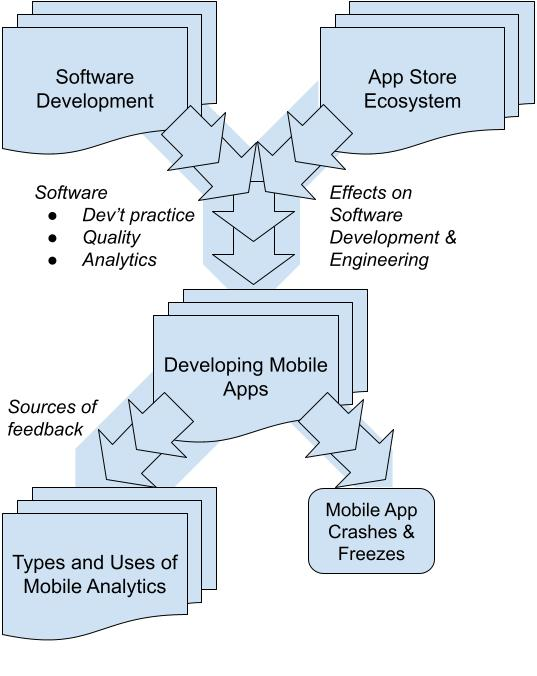
\includegraphics[width=\textwidth]{images/my/related-work-chapter-structure-27-jul-2022b.jpeg}
    \caption[Structure of this related work chapter]{Structure of this related work chapter\\ Source: \href{https://docs.google.com/drawings/d/1DosM__BfTGqoIYkkkltbyDreCT5wYC1Z0mR9i1ZSxWc/edit?usp=sharing}{Google Drawing}, access limited to collaborators to this thesis.}
    \label{fig:related-work-chapter-structure}
\end{figure}

\section*{Notes on the proposed tactics and topics for the related work chapter}
Marian suggests I aim for writing brief, one-paragraph summaries and apply the T tactic of the broad literature, the top bar of the T are the many and various papers on a topic, and I'm picking these ones that are most directly germane to my research which become the vertical bar of the T.\pending{I'm still currently more verbose than this :(} 

Marian also suggested I might end up with two or a maximum of 3 levels of Ts. The higher level would be on Software Quality Improvement. The lower level would be on mobile analytics.

Where others have done similar work they've done so in other ways eg MSR rather than focusing on the development teams. When I observed the teams the effects of the processes, artefacts, and the tools emerged. This is why I've picked these 3 aspects and 6 perspectives. 

\subsection*{Some notes on the methods used for the literature review}

\begin{figure}
    \centering
    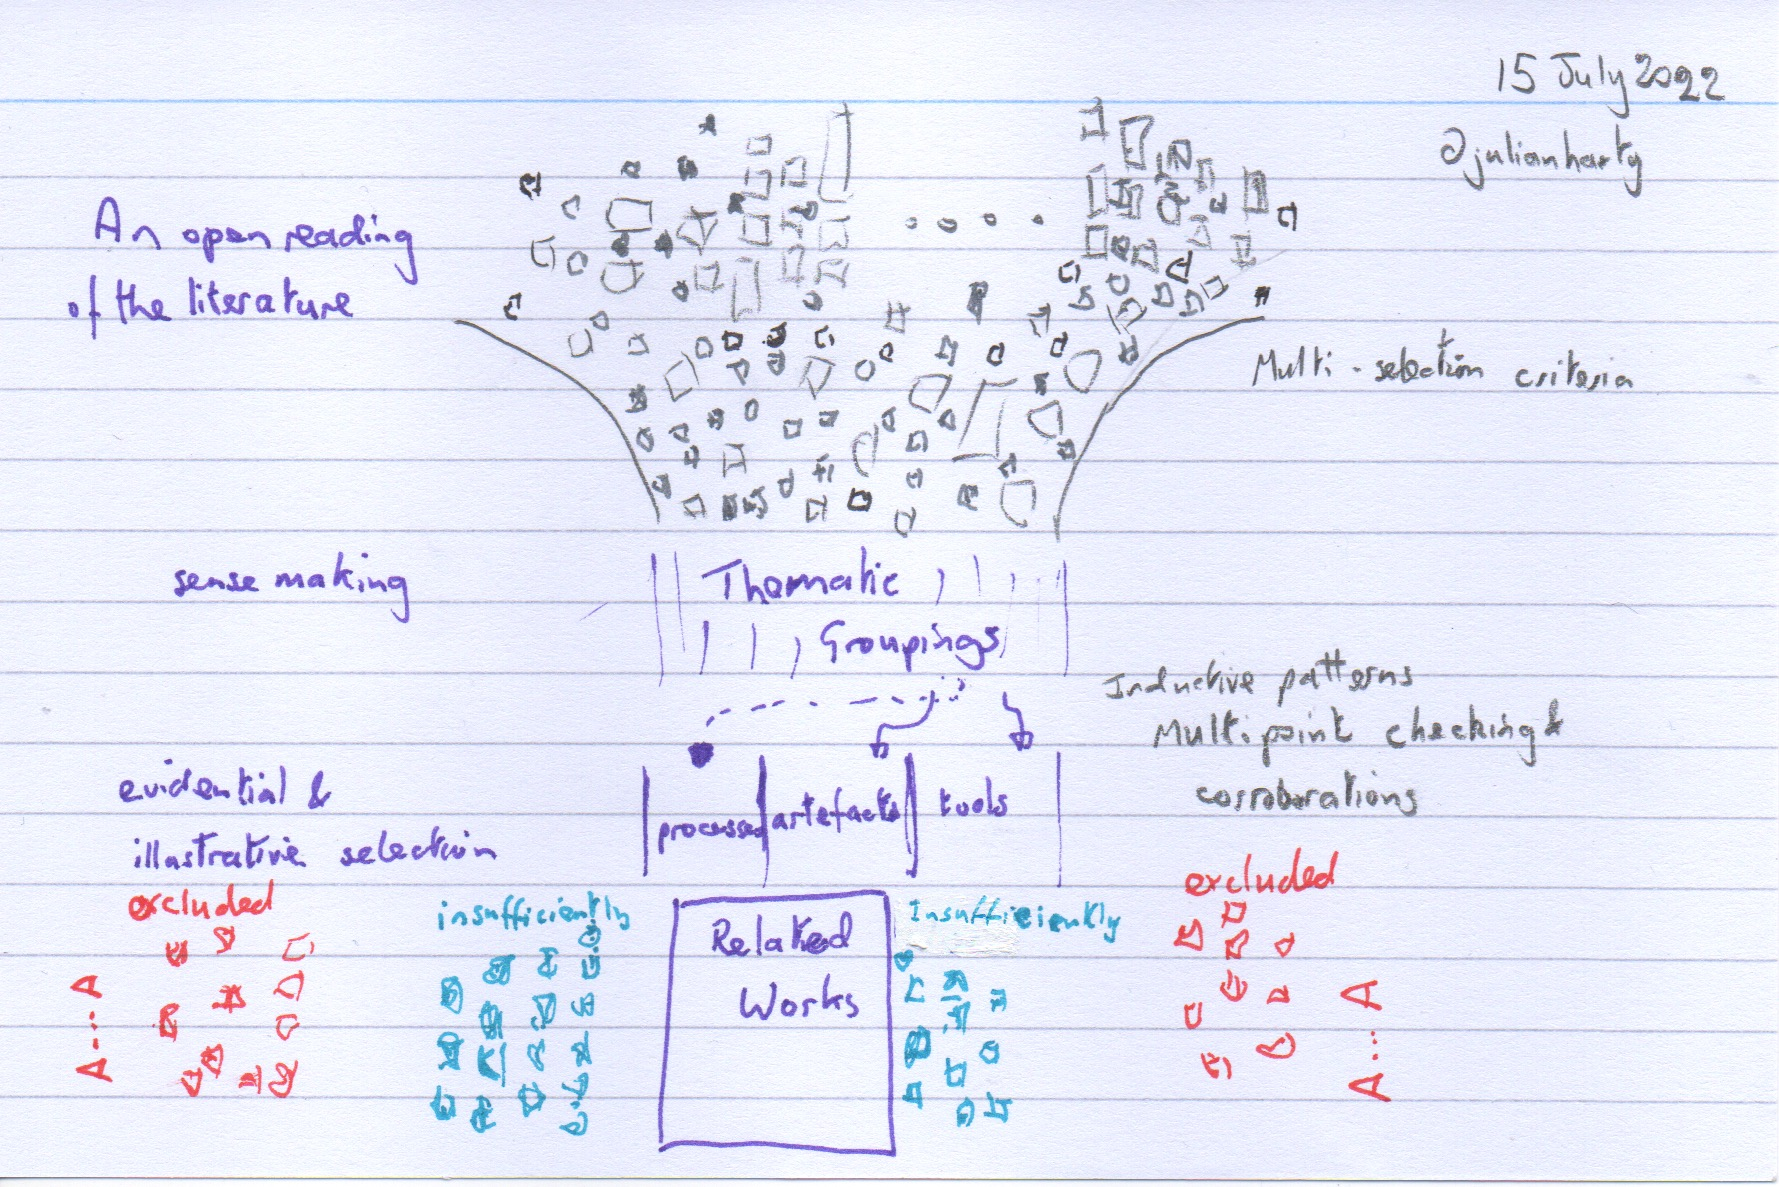
\includegraphics[width=\textwidth]{images/rough-sketches/literature-review-overview.jpeg}
    \caption{Overview of the literature review process and outcomes}
    \label{fig:literature-review-overview}
\end{figure}

Figure \ref{fig:literature-review-overview} illustrates my approach to researching prior work in the use of mobile analytics by app developers in order to measure and improve the stability/reliability of their mobile apps in the field/in the wild. Various searches, including keyword, tags, and related items, were incorporated into the searches. Initial sources included Google Scholar to find the more research oriented materials and Google Search particularly for grey materials, helped provide initial material to seed further searches. Specialist search tools were used where sites provided them, for instance on stack exchange sites such as StackOverflow, GitHub.com, acm.org, ieee.org, and medium.com their respective search engines were used frequently. Where practical copies of material has been preserved privately and backed up using at least one commercial, paid-for, cloud file storage service.

Multi-selection criteria are used to select material that appears of interest, relevant, and plausible. Generally bibliographic entries were obtained and these where checked for accuracy and completeness. Grey material seldom has a bibliographic entry, these were created, generally by hand, and preserved.

Through a process of sense-making, cross-checking, and corroborations various thematic groupings emerged together with potential relationships between the thematic groups. On reflection three clearly distinct and vital aspects emerged in the related work - the development practices used by mobile app developers, the artefacts they create and maintain, and the mobile analytics tools the developers use. These were further refined into six perspectives, using a three-by-two matrix: the x-axis incorporates the three aspects of processes, artefacts, and mobile analytics tools; the y-axis focuses on the current \emph{what is}, and \emph{what might be} in terms of making improvements.\pending{Arosha suggested three pillars which sounds good.}

The research materials and the bibliographic entries are maintained online. The most relevant ones are included in this thesis, many more are maintained in an `outtakes' folder, for example as `fieldstones'~\citep{weinberg2006weinberg} or in an insufficiently-related-works chapter. There's also an `excluded biography' file which helps reduce unnecessary repetition or groundhog day like practices. In the figure (\ref{fig:literature-review-overview}) the two \texttt{A ... A}'s wraps around - excluded works and insufficiently related works are similar distanced to this related works chapter.

In reading the literature various \textit{false friends} emerged, papers that first appear relevant because of their titles and/or abstracts but turn out to be on very different topics. 
Knowing about the concept of false friends and having pragmatic strategies to deal with them is important to avoid misunderstandings or misleading application of their work, 
based on \citep[p. 1833]{chamizodominguez2002_false_friends_their_origins_and_semantics_in_some_languages}. 
\citet{shaw1989_comparing_conceptual_structures__consensus_conflict_correspondence_and_contrast} uses the term 'conflict`, where, \emph{``experts use [the] same terminology for different concepts"}~\citep[p. 3]{shaw1989_comparing_conceptual_structures__consensus_conflict_correspondence_and_contrast} (and, indeed, using their terminology here there is a `correspondence' where experts use two terms to describe the same concept e.g. `false friends' and `conflict' both describe the same concept.). For this research my work was limited to recognising false friends and identifying some examples. 

So somehow I should aim to have the chapter structured with the following topics:\pending{This is a note to myself and needs replacing as I refine the chapter.}
\begin{enumerate}
    \item \textbf{Software Quality [Improvements] for mobile app developers}: Software Quality has been a contested topic for decades with no single accepted coherent agreement on what form(s) it takes, how software quality is measured, etc. Then comes the similarly vexed challenge of determining the concept and application of improvement in the quality/qualities of software. 
    \item \textbf{Mobile Analytics}: Research into \textbf{Processes, artefacts, and tools} necessary when using mobile analytics for improving software quality/qualities. These groupings emerged during the analysis of the literature and through understanding the practices of app developers.
    \begin{itemize}
        \item \textbf{Processes}: a.k.a. Analytics in Use - research into the processes developers use when they use mobile analytics
        \item \textbf{Artefacts}: things the developers create and maintain as part of their development work. Some of these are generated, in particular the app binary that is destined for end users once delivered by the app store.
        \item \textbf{Mobile Analytics Tools}: that the app developers use are worth researching in order to learn about their characteristics.
    \end{itemize}
\end{enumerate}

\subsection*{Software Quality Improvements for mobile app developers}
Here topics might include the measures that have been used by app developers to measure software quality - as confirmed by research literature and grey materials. I suspect this is where I'd include sources of information about software quality (\secref{rw-sources-of-info-on-software-quality-for-devs-of-mobile-apps}).

\subsection*{Development Processes for mobile apps}
Here topics include how the developers are perceived to work when they develop mobile apps, how they spend their time, how they structure and organise their work, etc. I suspect software testing fits here as well as how devs make mobile apps (the artefacts e.g. build scripts would go in the artefacts section).

\subsection*{Artefacts for mobile apps}
There's no end of research on artefacts from various subsets of opensource Android projects. Quite how well these reflect the population of shipping mobile apps (in Google Play in particular) is open to discussion. I can potentially include my joint research on logging practices as we aimed to only analyse projects where the codebase was actively maintained, etc. Research into logging practices by devs might also fit here (however how they use logging would be part of the section on development processes).

\subsection*{Mobile Analytics (and Mobile Analytics tools)}
I think it's germane to include research on the use of mobile analytics and any research into the tools, including the SDKs, data leakage, privacy, etc.

\subsection*{Thoughts on the above organisation of the related works}
As I've written the notes for each of the previous subsections I've had several instances where I've written about a single topic split across processes and artefacts. Perhaps it'd be better to keep the topics together and then summarise the topics by explaining there's a key distinction between the artefacts that exist and how they're used in practice. If so, then the alignment with the six perspectives would occur towards the end of this chapter rather than being used throughout. Let's see.

 % Moved the content to a separate file to reduce noise for the reader of the chapter in latex.


\section{Software Development}~\label{rw-software-development-section}
%%% Rationale for including this topic 
Mobile apps are developed using similar practices to other modern software projects, however there are key distinctions/differences such as: the build, packaging, and release processes (which are relatively similar to those for software apps generally), how analytics is designed, implemented, and how analytics works all differ. There are also nuances in the effects of software quality as measured by the app store which are important for us to be aware of.\sidenote{I,R,123456,C,G}

This section, and associated subsections, provide context for the more specific domain of mobile apps, covered in \secref{rw-developing-mobile-apps-section}~\sidenote{As an observation there appears to be little research into desktop apps, such as those available on MacOS. However, this is outside the scope of this research.}.
 
This section covers the following topics: \secref{rw-software-development-practices-topic}, \secref{rw-software-quality-including-measurement-topic}, and \secref{rw-software-analytics-topic}.

\subsection{Software development practices}~\label{rw-software-development-practices-topic}
Jez Humble is a well respected leader in modern software development practices who popularised the concepts of Continuous Delivery and DevOps. In \sidecite{humble2018_continuous_delivery_sounds_great} he argues the benefits of using continuous delivery to reduce risks and transaction costs, to create fast feedback loops, and work in small batches. He also believes it can be applied to any software and any domain. He concludes: \emph{``This, in turn, increases the quality of products, allows developers to react more rapidly to incidents and changing requirements and, in turn, build more stable and higher-quality products and services at lower costs.''}~\sidenote{[p. 39, \emph{Ibid}]}. To be successful in applying continuous delivery Humble identifies the importance of continuous, daily improvement and constant discipline to seek higher performance.\sidenote{I,R,123456,C,G} 

Can we assume continuous delivery is suitable for mobile apps and can be applied by developers of those mobile apps? Not necessarily: in an app store, deliveries are packaged into a software release that needs to be approved by the app store, the release needs to be accepted by end users as a replacement for a previous release of the app, and all this takes time. Existing research into releases in app stores, in \secref{rw-managing-releases-in-app-stores-topic}, provides context for where and how mobile analytics might make a useful contribution.\sidenote{I,R,123456,C,G}

\subsection{Software quality, including measuring software quality}~\label{rw-software-quality-including-measurement-topic}

Early work compared two approaches to software testing - debug testing and operational testing~\sidecite{frankl1997choosing_testing_for_reliability}. Their research considered the two approaches including their efficacy at improving reliability of the software being tested. This work challenged the focus on faults which they stated was nebulous and not necessarily the best term to use to describe what happened when failures were detected or when changes were made to 'fix' the code that led to the failures. They introduced the notion of \emph{failure regions}, which could be \emph{``eliminated by a program change''}~\sidenote{[p. 70, \emph{Ibid.}]}. This research and associated concepts align well with the use of mobile analytics to identify failures, and failure regions that are detected by mobile analytics and potentially addressed by changes to the program \emph{i.e.} the mobile app. We will revisit this paper in \secref{rw-mobile-app-crashes-topic}.\sidenote{I,R,123456,C,G}

The authors discussed the potential perils of relying on the judgement of people involved in debug testing (testing to maximise the faults found in a given period). They referenced~\sidecite{basili1994_software_process_evolution_at_the_sei} where testers who focused on `testing' over-estimated their abilities to find all the faults in a program. To counter the peril they proposed comparing the effectiveness of testing by using operational profiles~\sidecite[][p. 77]{frankl1997choosing_testing_for_reliability}. Although their research predates mobile apps, smartphones, and mobile analytics their perspective appears relevant and suitable. The comparison in terms of the effectiveness of testing could be operational results from mobile analytics reports.\sidenote{I,R,123456,C,G}

Another germane concern raised by Frankl \emph{et al} is the potential for debug testers to confuse \emph{``between detecting failures and achieving reliability.''}~\sidecite[][p. 77]{frankl1997choosing_testing_for_reliability}. This has been corroborated by my experiences in Industry where testing and testers often focus on regression testing and feature testing without considering, or factoring-in, the effects of the software being used.\sidenote{I,R,123456,C,G}

%Measuring software quality

One of the challenges has been to find ways to measure beyond an app, to behaviours that are externally observable but not easy to measure within an app, for instance how long the app takes to start from being launched. Unresponsiveness of software is a particular concern for mobile apps where apps stop responding for longer than deemed acceptable. Google Android coined the term \Gls{anr} for when the application stops responding. One of the challenges has been how to detect and measure these, particularly remotely on end-user devices.\sidenote{I,R,123456,C,G} 


\subsection{Software analytics}~\label{rw-software-analytics-topic}
Software analytics includes the use of analytics to measure and potentially improve processes, products, and software tools. Some of the early published research came from Microsoft Research. For example, Buse and Zimmerman wrote a short paper in 2010 which helped establish the field of:~\emph{``Analytics for Software Development"}~\sidecite{buse_analytics_2010}. The first figure in that paper is reproduced here as~\ref{fig:software_analytics_buse_and_zimmerman_2010}. As an observation, they derived that figure from a more general business-focused diagram in Davenport and Harris's book~\emph{``Analytics at work: Smarter decisions, better results"}~\sidecite[][p. 7]{davenport2010analytics_at_work}, so this figure appears to be broadly applicable once it has been customised.\sidenote{I,R,123456,C,G} %,  in Figure 1.1, titled\emph{``Key questions addressed by analytics"} and found in page 7 of ~\sidecite{davenport2010analytics_at_work}). 

\begin{figure}
    \centering
    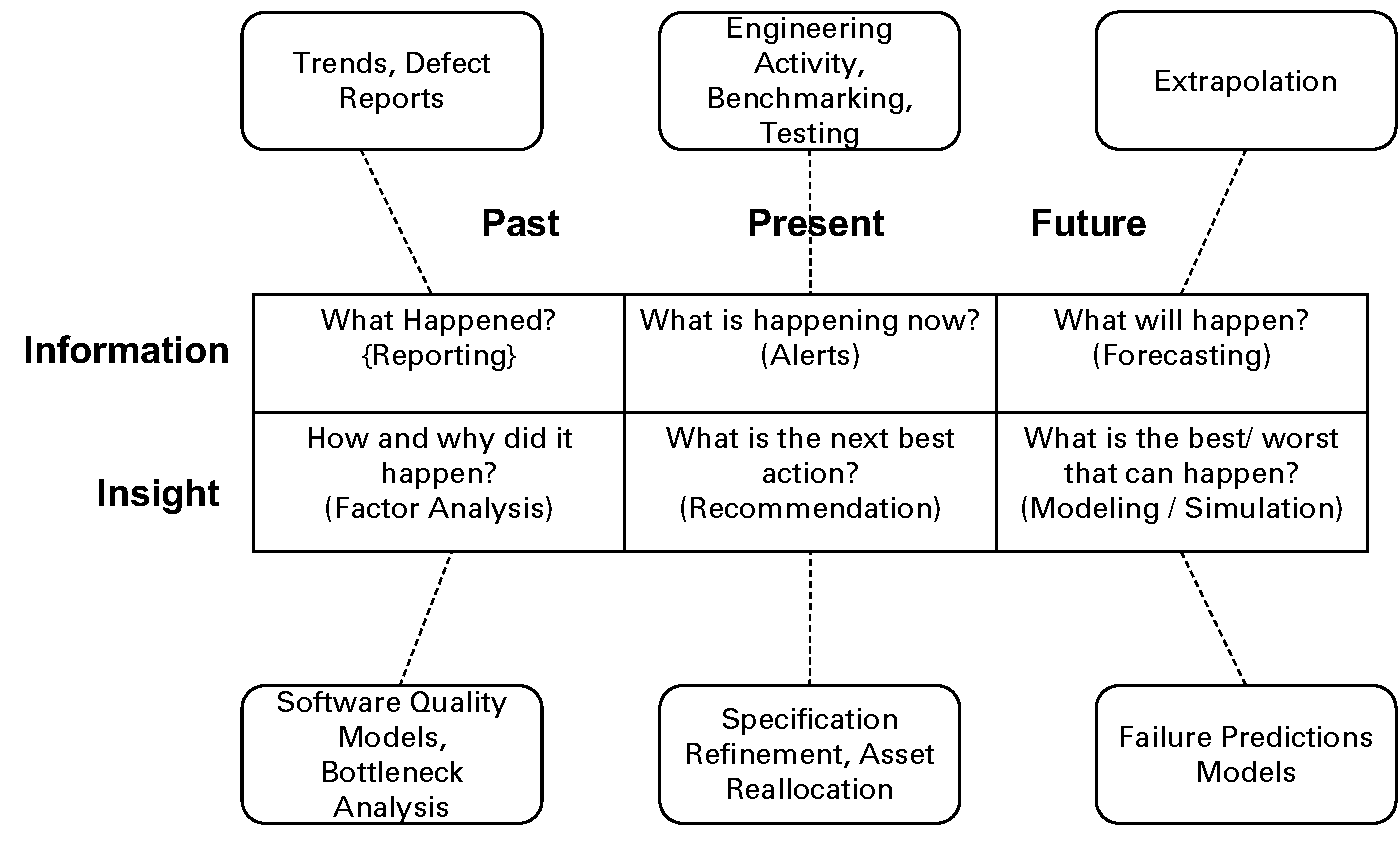
\includegraphics[width=\linewidth]{images/related-work/buse_and_zimmermann_2010_figure_a.pdf}
    \caption{Software Analytics, Buse and Zimmerman (2010)}
    \label{fig:software_analytics_buse_and_zimmerman_2010}
\end{figure}


In the Buse and Zimmermann paper they \emph{``distinguish between questions of information which can be directly measured, from questions of insight which arise from a careful analytic analysis and provide managers with a basis for action.''}~\sidecite[][p. 78]{buse_analytics_2010}. This is an important distinction. In this research the insights  are also pertinent to app developers, rather than being limited to managers.\sidenote{I,R,123456,C,G}

\subsubsection{Information needs}~\label{rw-information-needs-research}
Development teams comprise many roles including development managers and software developers. As Microsoft discovered these two roles have different information needs in terms of software development analytics~\sidecite{buse2012_information_needs_for_software_development_analytics}. They asked 110 Microsofties, a mix of development leads and managers, about their use of software development analytics, none were identified as working with mobile apps or Microsoft's then current mobile operating system or platform (p. 989).\sidenote{I,R,123456,C,G} 

Both the managers and the development leads agreed that \emph{``it [is] more important to understand the past than try to predict the future; echoing George Santayana, ``those who cannot remember the past are condemned to repeat it.''''} (p. 990). From Figure 4 in their work (p. 991), Failure Information (\emph{``reports of crashes or other problems"}) is in the top 3 that the development leads would use and top for managers when making decisions relevant to their engineering process. \myindex{Telemetry} would be used by approximately 80\% of development leads and 90\% of managers in the survey. The respondents used crash reports in their work and presumably these were considered to be part of software analytics given they were mentioned in this research. The survey did not appear to discuss software quality, reliability, or the use of software analytics (or telemetry) to improve the quality of their processes, artefacts, or analytics tools. They did consider data quality which was important to the respondents.\sidenote{I,R,123456,C,G}

Participants confirmed that analytics could help them \emph{``monitor a project; know what's really working; improve efficiency; manage risk; anticipate changes; evaluate past decisions.''} (p. 989).\sidenote{I,R,123456,C,G}

\begin{figure*}
    \centering
    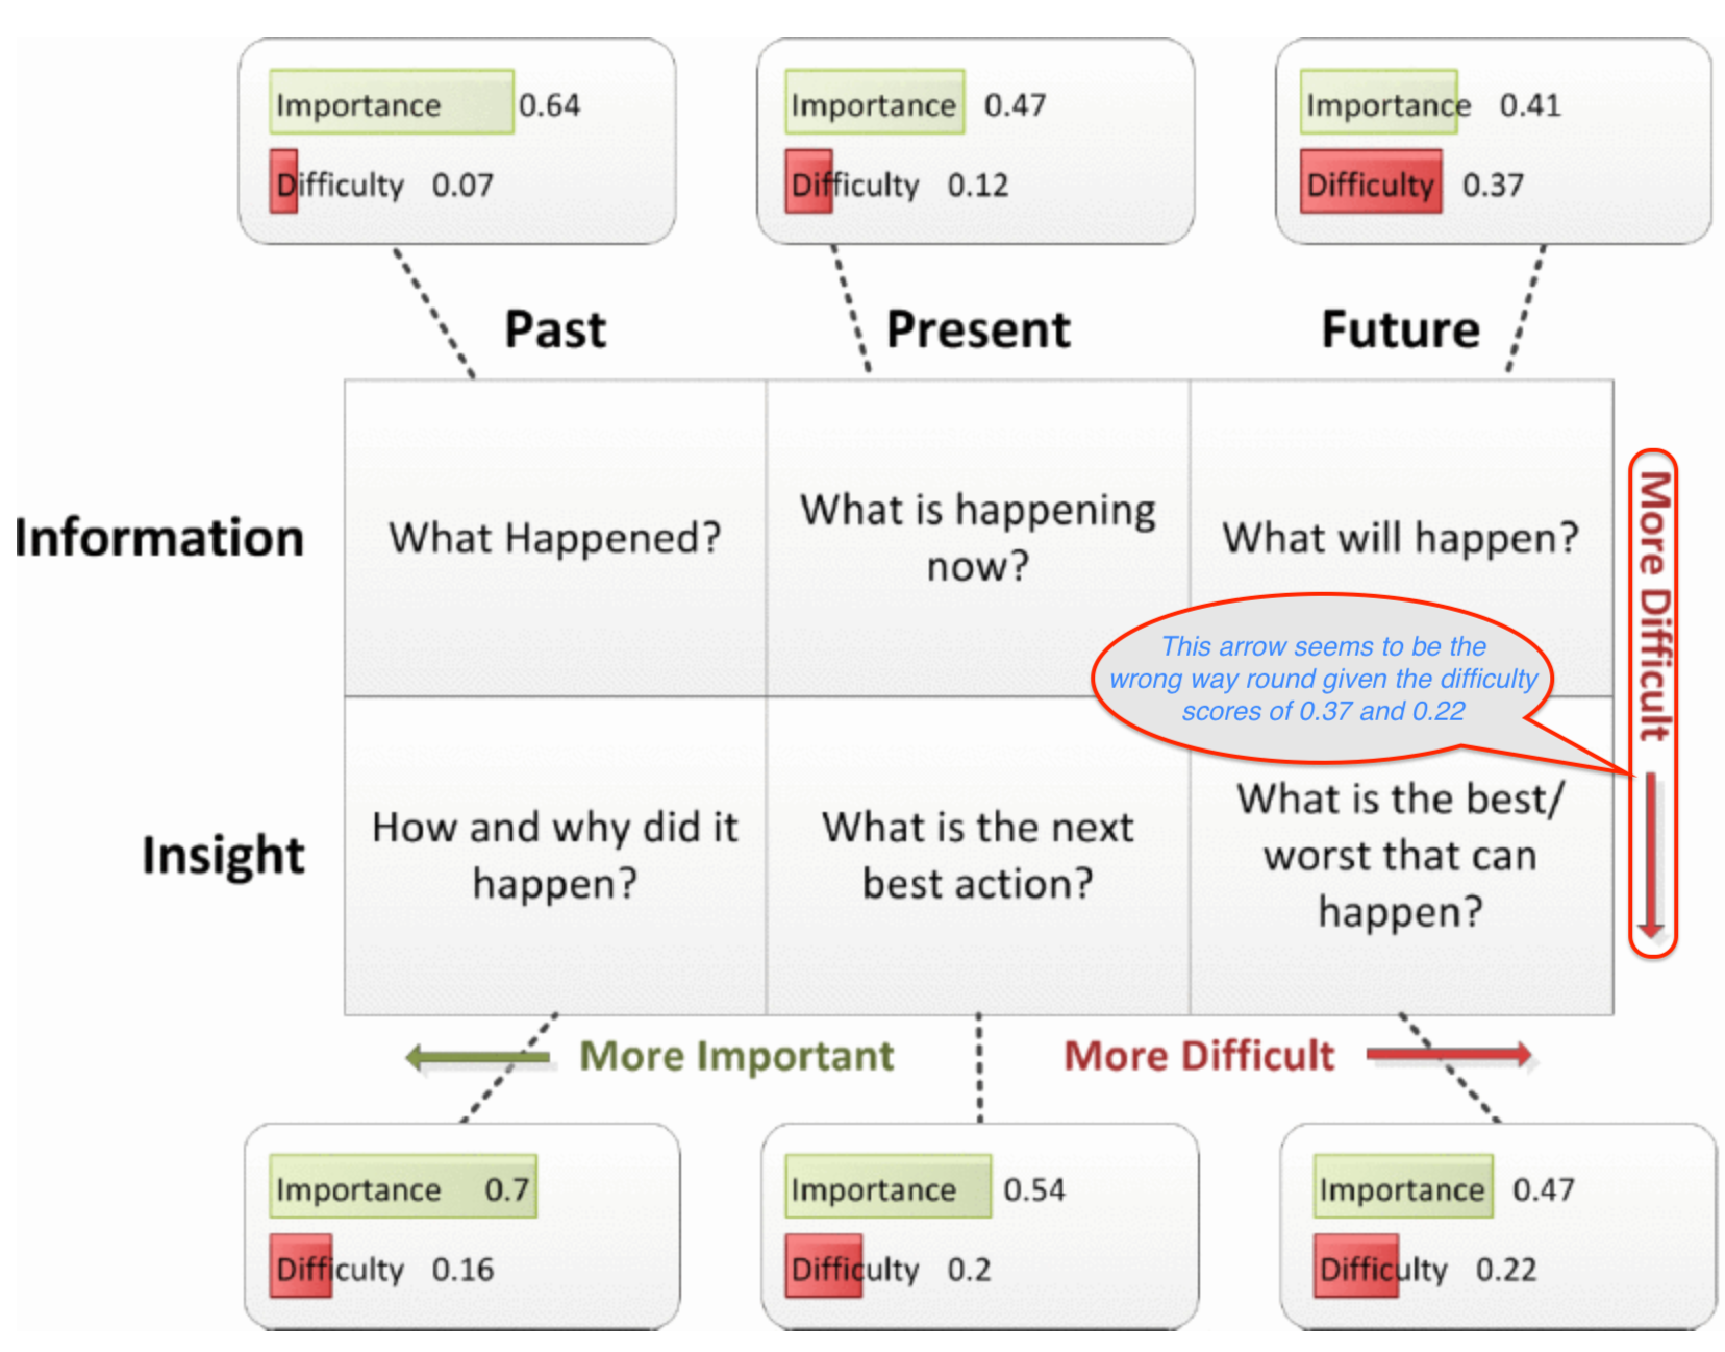
\includegraphics[width=\linewidth]{images/related-work/buse2012-edited-figure-2.pdf}
    \caption[Analytical questions, adapted from \cite{buse2012_information_needs_for_software_development_analytics}]{Revised Figure 2 from \cite{buse2012_information_needs_for_software_development_analytics}}
    \label{fig:buse2012-edited-figure-2}
\end{figure*}

Oddly, Figure 2 in their paper seems to have a mistake in the direction of More Difficult from Information to Insight, see~\ref{fig:buse2012-edited-figure-2}.

\emph{``The landscape of artifacts and indicators in software engineering is well known, but the concrete decisions they might support are not. We conjecture that understanding how managers and developers can make use of information is critical to understanding what information should be delivered to them."} (p. 992). 
My research somewhat inverts this by looking at what's being delivered in terms of commercial, pre-existing mobile analytics and considers how that information has been used to improve the reliability of the mobile apps that were the source of the raw information.\sidenote{I,R,123456,C,G}

Overall, their focus seemed to be more on the code than the product of the code (the apps, services, and qualities of those services those apps provide to end users). Unasked and unanswered in their work were : what information do mobile app developers need in terms of: improving their practices, the reliability of their apps, and the analytics tools and services they use? and, how can the developers make good decisions in this area?\sidenote{I,R,123456,C,G}

A much more recent paper, published on arxiv.org performed a \Gls{slr}~\sidecite{caldeira2020_software_development_analytics_in_practice_a_slr}. All the accepted 42 studies were aimed at developers (p. 10). Many of the papers included App Stores (p. 10) and the majority of the selected papers were from the Empirical Software Engineering Journal~\sidenote{\href{https://www.springer.com/journal/10664}{www.springer.com/journal/10664}}, yet none of the papers were identified with mobile analytics or crash reporting despite these two highly relevant criteria.\sidenote{I,R,123456,C,G} 


\subsubsection{Software analytics tools}~\label{rw-software-analytics-tools-research}
Software analytics generally involves software that is used as a tool to analyse whatever the data is. The tool may be limited to reporting based on existing data or it may include data collection. The tools may range from a spreadsheet editor, through heavy-duty yet data agnostic tools, to custom and highly tailored reporting systems. In this research the focus is on the custom and highly tailored reporting systems, generally packaged with the respective data collection \Gls{sdk}, services, \emph{etc.}\sidenote{I,R,123456,C,G}  

In terms of research into software analytics and tools used to provide analytics about the use of software, Microsoft's work with their \Gls{wer} is particularly of interest.\sidenote{I,R,123456,C,G} 

\newthought{Learning from Windows Error Reporting: }
The data collection and analysis of Android Vitals shares various similarities with Microsoft's \acrfull{wer}\index{Windows Error Reporting (WER)}. \Gls{wer} from a research perspective is described in an article in 2011~\sidecite{kinshuman2011_debugging_in_the_very_large} and a longer conference paper from 2009~\sidecite{kinshuman2009_debugging_in_the_very_large}.\sidenote{I,R,123456,C,G} 

Similarities include both mechanisms being designed to work effectively at scale of at least a billion end-user machines and devices, data capture including capturing crash data, and the use of error statistics as a tool in debugging.\sidenote{I,R,123456,C,G}

Differences include the platform (Android) which lacks automatic diagnosis (which \Gls{wer} provided). And, most relevantly, Google provides several million third-party developers with access to data for the apps they are responsible for and provides them with various comparative analytics of the technical performance of their app compared to those apps of their peers. (Microsoft provided 700 third-party developers, for instance of device drivers, with WER information, and the paper provides a concrete example of how one vendor addressed the top 20 reported issues for their code, and how the fixes percolated out to the end users and halved the percentage of all kernel crashes attributed to that vendor (from 7.6\% to 3.8\%)). Statistics-based debugging, described in these papers, was used in Microsoft's WER and may also apply when developers use mobile analytics.\sidenote{I,R,123456,C,G}

\newthought{Beyond Microsoft: }
Microsoft are not unique in publishing research about the use of software analytics. A company, Softeam, used a software analytics platform to collect feedback from their customers and systems with the aim of improving the software quality of their systems~\sidecite{bagnato2020_challenges_and_benefits_from_using_software_analytics_in_softeam}. They use \href{https://github.com/q-rapids}{github.com/q-rapids}~\sidenote{A ``Quality-aware rapid software development. H2020 Project (Grant no. 732253)''.}. There are additional publications of interest listed at \href{https://www.q-rapids.eu/publications}{www.q-rapids.eu/publications}, however they are excluded from this thesis as they do not further contribute to this research.\sidenote{I,R,123456,C,G}


\subsubsection{Interpreting analytics data}~\label{rw-interpreting-analytics-data-research}
As Microsoft noted, interpreting the data in order to provide a basis for action is a necessary facet of what development teams need to do. Here we consider two aspects: connecting, or combining, failures with software analytics, and \emph{caveats} with software analytics.\sidenote{I,R,123456,C,G}

\newthought{Connecting failures with software analytics: }
In a short paper~\sidecite{kidwell2015_toward_fault_taxonomy_application_of_software_analytics}, the authors propose combining fault classification and software analytics for five types of decisions. These are: targeting testing, release planning, judging stability, targeting training, and targeting inspection of software. Their paper provided initial indicative evidence of their proposals through evaluation of changes to source code for the Eclipse software. It also discussed the measurement of refactoring to provide more accurate and relevant measurements of the efficacy of the refactoring. This work is relevant in terms of aspects such as judging stability and targeting inspection of the software. Their research did not consider approaches to improve mobile apps through mobile analytics.\sidenote{I,R,123456,C,G} 

Failure data mined from software analytics tools such as crash reporting tools might help to bring their concepts and ideas to life.\sidenote{I,R,123456,C,G}

\phantomsection
\newthought{Caveats with software analytics: }~\label{rw-caveats-with-software-analytics-topic}
Using software analytics leads to several \emph{caveats} to consider the `so what' aspects and whether the research is being done well. For our research to be applicable it needs to pass two tests. The first test is to answer: 
\emph{``Software Analytics, so what?"}~\sidecite{menzies2013_software_analytics_so_what}. The second is to avoid doing or publishing poor quality work~\sidecite{menzies2019_badsmells_in_software_analytics}!\sidenote{I,R,123456,C,G}


\subsection{Summary}
Software development research has a bearing on mobile app development, a topic we investigate shortly in \secref{rw-developing-mobile-apps-section}, and software analytics also has a bearing on this. Nonetheless the general research we have investigated so far does not consider app stores or their effects on software development and engineering practices. App stores have been researched extensively so we will investigate pertinent research in the next section.\sidenote{I,R,123456,C,G}

%Traditional software analytics tools are not the only source of information researchers have also looked at information from app stores and the effects of app stores on mobile apps, therefore these will be investigated in the next section.   


\section{App Stores and their Effects on Software Development and Engineering}~\label{rw-app-stores-and-their-effects-on-software-development-and-engineering}
% Software developers have flocked to develop mobile apps as that's where billions of users find and use software. In the era of mobile apps before smartphone app stores the device manufacturers and the carriers were the dominant parties. Developers provided their apps directly and/or via carriers and/or a variety of third-party app stores. The ecosystem shortly before the point of inflection is nicely captured in \sidecite{lin2009_os_battle_in_the_ecosystem_of_smartphone_industry}. 

App stores are part of an ecosystem that provides and enforces rules that also constrains various choices. They also allow various freedoms for the participants within the ecosystem. The ecosystem needs to sustain competition~\sidecite[][p. 94]{KAPOOR2021_socio_technical_platform_ecosystems_etc} and revenues. The two largest app stores, Google Play and Apple's App Store, each have their own development platform including an \Gls{ide} and additional software tools, various \Glspl{sdk}, developer programs, release processes, pricing and revenue rules, and so on. 
%They can effectively severe the connection between developers and their market.
Pivotal effects include: the app approval process (which gates any release of the app to the general user population), rules and restrictions on what the binary contains, the signing process, how the app is packaged/bundled. Another pivotal effect is how app quality is measured and assessed by the app store, at least, as app developers have a vested interest in having high quality apps as determined by the app store.\sidenote{I,R,123456,C,G}

App Stores behave as intermediaries between developers and the users of their software. They make various aspects more transparent including pricing, information about the apps, releases, and ratings \& reviews. There are hundreds of thousands of developers of Android apps according to various sources (320,000 in 2017~\sidecite{wang2017_exploratory_study_of_the_mobile_app_ecosystem}).\sidenote{I,R,123456,C,G} %TODO add the reference to a larger estimate.

In an App Store, first the developer then the app store are involved in making a release available to some or all of the user population. There are various competing factors that affect when would be a good time to make a release. Too few and an app may be considered stale or neglected, too many and users may balk at the seemingly endless updates and communications costs. This topic is covered in \secref{rw-managing-releases-in-app-stores-topic}.\sidenote{I,R,123456,C,G}  

This research primarily focuses on the Android ecosystem and the Google Play store - the combination is the preeminent platform in terms of userbase, reach, and platform analytics provided to app developers. However, recognising that these are other ecosystems, this research also includes investigations of several additional platforms and app stores, \emph{e.g.} the Window Phone platform with Microsoft's app store and Huawei's app store for Android, where they contribute to this research.\sidenote{I,R,123456,C,G} 

App stores and their ecosystem have affected the lives of billions of end users and millions of software developers. They have become the primary route to market for many app developers and their organisations (exceptions include companies who developed strong businesses elsewhere such as Amazon and Netflix). 
From a research perspective, in 2010, early papers were published on various effects of app stores on academic research \emph{e.g.} how app stores addressed some of the previous constraints such as reaching more users and facilitating the distribution of the apps and feedback from those users.\sidenote{I,R,123456,C,G} 

Cramer \emph{et al} discussed aspects of \emph{research in the large} and in particular for my research the importance of ``playing by the rules"~\sidecite{cramer2010_research_in_the_large_app_stores}. This research identified the importance of what happens when developers were deemed not to play by the rules (covered in \secref{rw-power-dynamics-topic}) and this research has been shaped to play by the rules of the app store.\sidenote{I,R,123456,C,G} % Where practical through responsible disclosure of flaws found in 

Miluzzo \emph{et al} introduced other relevant research aspects, \emph{i.e.}  ongoing concerns such as how to assess correctness when there is no \emph{``ground truth"} - a challenge when evaluating mobile analytics for shipping apps; and a software development model of \emph{``deploy-use-refine"}~\sidecite{miluzzo2010research_in_the_app_store_era}, where app development refines the app based on data gleaned from usage of the app. Their paper even explained how a silly mistake caused their app to crash where the app store then delayed the new release of the app by several weeks. Even in 2010 crashes adversely affected the app store's perception of an app.\sidenote{I,R,123456,C,G} % Their work on CenseMe received an ACM Test of Time award, see https://www.cs.dartmouth.edu/~campbell/page-3/


In more recent research, Wang, Li, and Gao~\sidecite{wang2019_understanding_the_evolution_of_mobile_app_ecosystems_a_longitudinal_measurement_of_google_play} provided an helpful longitudinal evaluation of the Google Play ecosystem and raises interesting questions and observations about Google Play. However, they did not seem to consider flaws, or the effects of flaws, in the app store's data collection, algorithms,\emph{ etc.}\sidenote{I,R,123456,C,G}

In terms of effects of app stores on software engineering practices there have been several seminal papers. %written by authors at UCL as part of their App Store Analysis Group~\footnote{http://www0.cs.ucl.ac.uk/staff/F.Sarro/projects/UCLappA/UCLappA.html} while it was active (until roughly 2019). 
%
Of these papers, the first~\sidecite{alsubaihin2019app_store_effects_on_software_engineering}, combined interviews with a survey to ask developers of their experiences of developing mobile apps and how those experiences differed with developing other software.\sidenote{I,R,123456,C,G}
%
Of the ten developers they interviewed a couple were for popular apps (800,000 downloads, 2,000 ratings, 1,000 ratings), the rest were for less popular apps.\sidenote{I,R,123456,C,G} % 0.1% ratings to downloads for a developer of 1M downloads app: https://www.quora.com/What-is-a-typical-ratio-of-reviews-to-active-users-to-downloads-for-iOS-and-Google-Play-apps

Their research identified automatic in-app crash reporting as the most frequent source of bug reports and the second-most frequently addressed in terms of bug fixes (end-user written bugs were addressed slightly more frequently)~\sidenote{[p. 10, \emph{Ibid.}]}.\sidenote{I,R,123456,C,G} 

Of particular interest was the discovery that the quality of the [source] code was the least important factor to build a successful app according to the survey results and furthermore the number of downloads were the highest measure of success according to the developers surveyed in this research~\sidenote{[p. 13, \emph{Ibid.}]}. Note: Google subsequently (but not necessarily because of this research) have placed a lot of focus on encouraging developers to improve the quality of their Android apps in Google Play.\sidenote{I,R,123456,C,G} 

Their research is one of several that discusses the gaming of app store ratings, such gaming is unsurprising given the importance placed on these ratings and particularly in having mobile apps with high ratings in the app store. Given their importance in the mobile app ecosystem, ratings and reviews are one of the topics covered in \secref{rw-sources-of-info-on-software-quality-for-devs-of-mobile-apps}.\sidenote{I,R,123456,C,G}

\emph{Future Trends in Software Engineering Research for Mobile Apps}~\sidecite{nagappan2016_future_trends_in_sw_eng_for_mobile_apps} focuses attention on the software development life-cycle, it does not investigate usage or operational aspects. Figure~\ref{fig:nagappan2016_future_trends_in_sw_eng_for_mobile_apps_figure_1_annotated} is an annotated version of their Fig. 1. \sidenote{[on p. 22, \emph{Ibid.}]} where the annotation, shown in purple in a bounded box, shows the key operational and usage areas their work did \emph{not} cover.\sidenote{I,R,123456,C,G} 


\begin{figure}
    \centering
    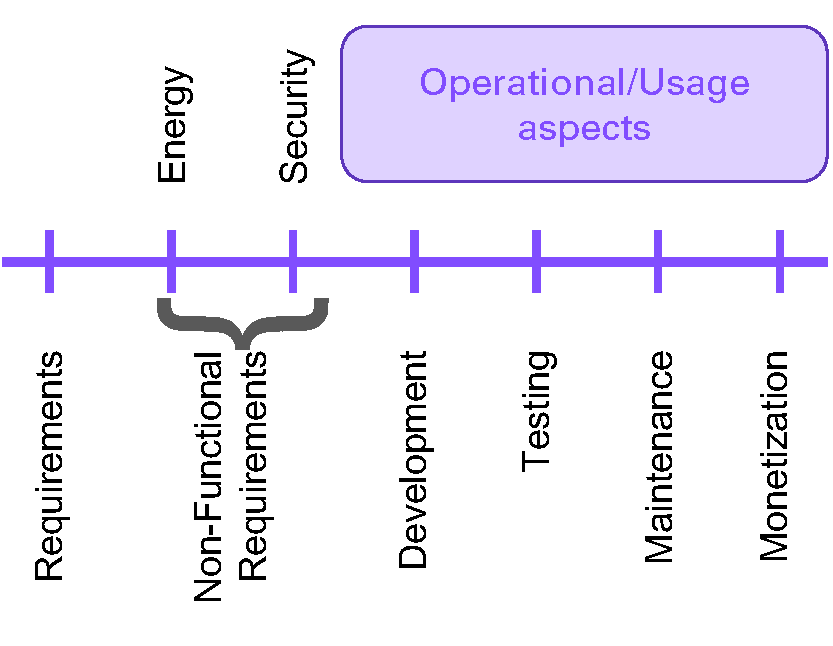
\includegraphics[width=\linewidth]{images/my/framework-for-presenting-the-state-of-the-art-in-sw-end-for-mobile-apps.pdf}
    \caption[Framework for presenting the state-of-the-art in software engineering for mobile apps, adapted from~\cite{nagappan2016_future_trends_in_sw_eng_for_mobile_apps}]{Annotated version of the framework for presenting the state-of-the-art in software engineering for mobile apps~\cite{nagappan2016_future_trends_in_sw_eng_for_mobile_apps}}
    \label{fig:nagappan2016_future_trends_in_sw_eng_for_mobile_apps_figure_1_annotated}
\end{figure}


Mining review data for various forms of data including requests for bug fixes as is using rating as an assessment of goodness. 
Figure~\ref{fig:nagappan2016_future_trends_in_sw_eng_for_mobile_apps_figure_2_annotated} is an annotated version of their Fig. 2 \sidenote{[on p. 23, \emph{Ibid.}]}. The annotations include feedback in the forms of ratings and reviews and in the form of mobile analytics. Various sources of information can be used by the development team, of these ratings and reviews are broadly researched, whereas device-level and app-level analytics have not been previously researched in the context of app stores.\sidenote{I,R,123456,C,G}


\begin{figure*}
    \centering
    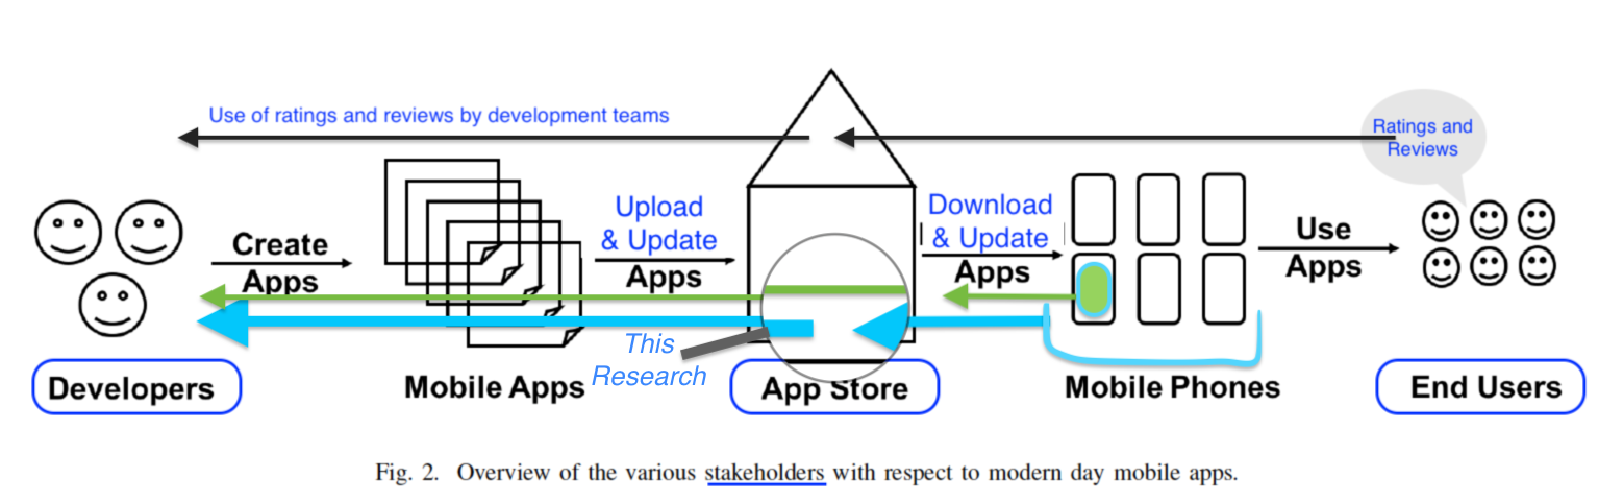
\includegraphics[width=\linewidth]{images/related-work/future-trends-in-sweng-for-mobile-apps-fig-2-annotated-with-highlights.pdf}
    \caption[Various stakeholders in the modern app store ecosystem, adapted from~\cite{nagappan2016_future_trends_in_sw_eng_for_mobile_apps}]{Annotated version of the various stakeholders in the modern app store ecosystem~\cite{nagappan2016_future_trends_in_sw_eng_for_mobile_apps}}
    \label{fig:nagappan2016_future_trends_in_sw_eng_for_mobile_apps_figure_2_annotated}
\end{figure*}
 

A key challenge identified is restricted access to data held by the app store. The only way they identified in their research was to gather historical information by continually mining the app store on a regular basis~\sidenote{[pp. 22-23, \emph{ibid}]}. Perhaps the authors weren't aware that developers of Android apps have access to various historical data about their apps including long term access to all the reviews of their apps. Details of how developers can download these and other reports, including the data structures, are available online~\sidecite{google_play_download_and_export_monthly_reports}.\sidenote{I,R,123456,C,G}

An area their work did not discuss is whether failure data could, potentially, be a form of requirements? (in a similar fashion to leveraging reviews in the app store to extract `requirements'). And similarly can complaints and failure data be combined to help developers prioritise issues they should consider addressing (the paper restricted the discussion to prioritising issues the developers should be \emph{testing} for).\sidenote{I,R,123456,C,G}

Finally in terms of this paper, they included two stakeholders, the developers and the end users. The app store (and the people and organisation who provide the app store) are also direct stakeholders in the ecosystem. There are additional indirect stakeholders including advertisers, researchers, and probably many others.\sidenote{I,R,123456,C,G} 

%
So far, we have considered various aspects of app stores and their effects on software development and engineering. Conspicuous by their absence is research into the provision and use of platform-level: mobile analytics, software release management tools, or pre-launch testing. There are several additional topics that are germane to app stores and their effects, these are covered in the following subsections.\sidenote{I,R,123456,C,G}


\subsection{Utility and Service Providers}~\label{rw-utility-and-service-providers-topic}
Developers use software and related services from various providers where the providers are the primary source of any updates. The providers may charge for their offerings and similarly they may mandate various behaviours from developers and their organisations who use the utilities and/or services.\sidenote{I,R,123456,C,G}

In the context of this research mobile analytics are provided as utilities and/or services by third-parties to app developers therefore it is useful to learn of pertinent research into the use of these utilities and services. Utilities include software tools, libraries, frameworks, and so on; and services may be provided either for some of these utilities or for additional capabilities, support, and so on. Some of the offerings are specific to mobile apps, however many include other platforms such as web sites and/or web apps. Of these examples, an understanding of the use of software libraries helps identify the proclivity of developers to use them and similarly services that apps use are particularly relevant.\sidenote{I,R,123456,C,G}


\subsection{Software libraries}~\label{rw-software-libraries-topic}
Developers can choose to use external libraries to generate revenue (ads)~\sidecite[][p. 407]{li2016_an_investigation_into_the_use_of_common_libraries_in_android_apps}, to \emph{ease the management of HTTP requests}~\sidecite[][p. 73]{belkhir2019_an_observational_study_on_the_state_of_rest_api_uses_in_android_apps}. Related work found 98\% of android apps used third-party libraries in their apps~\sidecite[][p. 218]{abdellatif2020_a_multi_dimensional_study_on_the_state_of_practice_of_rest_apis_usage_in_android_apps} and on average 41\% of android apps is contributed by common libraries~\sidecite[][p. 409]{li2016_an_investigation_into_the_use_of_common_libraries_in_android_apps}. Using the data in Fig. 5 of this paper (on p. 409) 5\% of the apps included Google Analytics and 2.6\% used Flurry analytics. Note: Industry data indicates mobile analytics are now incorporated in the vast majority of Android apps.\sidenote{I,R,123456,C,G}  

\subsection{Services used by apps}~\label{rw-services-used-by-apps-topic}
Two of the extremely popular categories of third-party libraries are advertising (ads)~\sidenote{According to AppBrain the majority of Android apps include at least one advertising library \href{https://www.appbrain.com/stats/libraries/ad-networks}{www.appbrain.com/stats/libraries/ad-networks}} and mobile analytics~\sidenote{And at least 80\% include Firebase Analytics alone, \href{https://www.appbrain.com/stats/libraries/tag/analytics/android-analytics-libraries}{www.appbrain.com/stats/libraries/tag/analytics/android-analytics-libraries}}.
In some ways app developers appear to be similar to their end-users - neither wants to pay up front for what they use.% TODO {Add research into the ratio of free to paid apps.} 
Typically service providers have at least one form of unpaid service offering that is either time- or volume-based. Many also have at least one paid-for service offering that has fewer restrictions than their unpaid offering.\sidenote{I,R,123456,C,G}


\subsection{Services used by developers: Device Testing Services}~\label{rw-services-used-by-devs-device-testing-services}
Remote device farms are good examples of services that at least some developers (and/or their organisations) pay for. They were used by development teams, including two of the app-centric case studies: \myindex{Kiwix} and \Gls{gtaf}\index{GTAF} for pre-release testing with the aim of finding bugs and crashes.\sidenote{I,R,123456,C,G}

Device test farms have been available commercially since around 2008~\sidenote{Based on the author's professional experience.}. Over the years different offerings have peaked and then either been acquired, retired, or disappeared.
Early research, written by one of the co-founders of a device testing service, \myindex{TestDroid}~\sidenote{TestDroid later became Bitbar which was later acquired by SmartBear Software.}, provided insights into the bug-finding abilities when tests were run on a mix of their devices~\sidecite{kaasila2012_testdroid_etc}. Whereas more recent research investigated the use of an in-house device farm based on the \myindex{Open-STF} project~\sidecite{klinsman2020_moraystf_a_novel_approach_for_requirement_definition_for_gsd_projects_in_a_mobile_ecosystem}.\sidenote{I,R,123456,C,G} 

Google, Amazon and Microsoft offer paid-for device farms as do various specialist businesses including \href{https://support.smartbear.com/bitbar/docs/about-bitbar.html}{SmartBear Software}. There have been a couple of public-good initiatives including Open Device Labs~\footnote{For example~\url{https://opendevicelab.com/},~\url{https://www.devicelab.org/}}; and Open STF~\sidecite{openstf_website} which is based on a set of opensource projects~\sidenote{\url{https://github.com/openstf/}{github.com/openstf/}} and enables teams and organisations to build their own device farms or use commercial offerings based on these projects~\footnote{For example~\url{https://www.headspin.io/}.}.\sidenote{I,R,123456,C,G}
% https://loadfocus.com/blog/tech/2018/04/building-your-in-house-device-farm-on-mac-os-using-openstf-for-android-testing/ 
% https://tech.mercari.com/entry/2019/02/18/173236 (on using HeadSpin and NimbleDroid).

A relatively dated paper about the then current device farm services provides a useful overview~\sidecite{starov2015_taas_for_mobile_apps_survey} but does not discuss pricing; and it predated the now popular service offerings by Google, Amazon, and others.\sidenote{I,R,123456,C,G} 

Device testing services are one approach used by development teams to increase the possibilities of finding bugs including failures of the app. However they do not necessarily find bugs and failures that affect end users in production, so they may not be sufficient by themselves.\sidenote{I,R,123456,C,G}


\subsection{Power dynamics}~\label{rw-power-dynamics-topic}
Grey literature is the main source of the imbalance in power between app developers and the app store, at least in terms of Google Play and Android apps in that store. I have selected four illustrative articles, by four different developers, of the 20+ related articles published on \href{https://medium.com/}{Medium} % More material is available on corporations on mining data from the public  from and via https://jilliancyork.com/
about how they lost access to their apps and in some cases their account.\sidenote{I,R,123456,C,G} 

In \textcite{martinez2019_google_just_terminated_our_startup_google_play_publisher_account_on_xmas_day} the termination of a personal Google Play account for an indirectly associated developer, via one of the employees of the small company, was attributed to the termination of that company's Google Play account. This story has ongoing updates that lists various developers who have had similar experiences. A similar experience was reported by \textcite{dodson2019_google_completely_terminated_our_new_business_etc} where apparently someone's associated account was the cause of Dodson's account being terminated. As Méa dry noted \emph{``google@play-store: sudo rm -rf org.mtransit.android*''} which happened abruptly within a few hours of Google sending automated email notifications to the developer. The reason given in the automated emails was the app was in violation of the ``Deceptive Behavior policy''~\sidecite{mea2019_google_just_deleted_my_nearly_10_year_old_app_etc}.\sidenote{I,R,123456,C,G} 

In these three instances the developer accounts were reinstated. In \textcite{marcher2021_how_google_terminated-a-developer} the account was not reinstanted and two of his clients also had their accounts terminated. As Marcher notes \emph{``I develop software not just for fun but also primarily for a living. This action not only deprives me of a substantial part of income, but it also forbids me for life to continue my work which is also my passion''}.\sidenote{I,R,123456,C,G} % See also https://medium.com/@appsrentables1/google-cancels-our-google-play-publisher-account-and-ends-my-familys-source-of-income-97d4e85cd046 and various others (20+ stories)

A word to the wise, at least one researcher known to the author discovered their developer account is no longer allowed to create Android apps after they uploaded some experimental apps Google disapproved of.\sidenote{I,R,123456,C,G}

\subsection{Developers and their app counts}
Before we leave the topic of App Store ecosystems and in particular a developer focused perspective on the ecosystem, the work of \citeauthor{wang2017_exploratory_study_of_the_mobile_app_ecosystem} looked interesting as it claimed to look at the Google Play store from a developer's perspective~\sidecite{wang2017_exploratory_study_of_the_mobile_app_ecosystem}. However, in practice they actually researched mappings between developers and the number of apps they had in Google Play Store. In other words, the paper concentrates on the characteristics of developers who have many apps in the app store rather than on the software development/engineering aspects.\sidenote{I,R,123456,C,G}

They estimated there were 320,000 developers, over half of the developers only released a single app. The paper main focus though is on the \emph{``the group of aggressive developers who have released more than 50 apps, trying to understand how and why they create so many apps''}. In terms of this research this paper provides some context on who writes the mobile apps in Google Play, and it provides an estimate of the population of developers (in 2017). However, it doesn't help us gain a better understanding of how developers apply and use mobile analytics or use app store data to improve the quality of their apps.\sidenote{I,R,123456,C,G}

\subsection{Summary} % Of app stores and their effects
App stores and their broader ecosystem, illustrated in figure \ref{fig:my_modern-mobile-app-ecosystem}, clearly affect software development and testing practices of app developers for that ecosystem. While telemetry\index{Telemetry} has been used to obtain and analyse crash data there is a gap in the research in terms of both \gls{glossary-platform-analytics} and in-app analytics. The next area of research is in developing mobile apps to investigate what pertinent research exists.\sidenote{I,R,123456,C,G}


\section{Developing Mobile Apps}~\label{rw-developing-mobile-apps-section}
Research into the development practices and mechanisms for mobile apps establishes various norms, characteristics, and habits, of app developers. Their work, collectively, is used by billions of people throughout the world. In terms of this research, understanding the development practices and mechanisms is vital. Developers also have a voice and hundreds have been interviewed to learn what's important to them, for example in \sidecite{joorabchi2013_real_challenges_in_mobile_app_development}. They also communicate through various artefacts they create and maintain, again these artefacts have been studied to learn about their work, for example in \sidecite{pascarella2018_self_reported_activities_of_android_developers}.\sidenote{I,R,123456,C,G}

% Some of the effects of their work in terms of software quality will be covered later in this chapter in \secref{rw-mobile-app-crashes-topic}.

Mobile apps need to be made and developers make them. There are various working practices, apps are made by visionaries, employees, amateurs, and communities. There are various activities involved including development, testing, release, and deployment.\sidenote{I,R,123456,C,G} % Figure~\ref{fig:my_mobile-app-makers} highlights these activities as part of the overall ecosystem.

% Many mobile app development teams would describe their development practices as Agile or based on along the principles of Agile development. % Solo app developers are less likely to use these practices, nonetheless there has been various research into adaptions of Agile and Scrum in attempts to suit them. Various examples are in the excluded-bibliography.
% Many of these people claim to be ``Agile" in their working practices.

5,000 commit messages (of over 1.8 million identified) were studied that were selected from 8,280 active opensource Android apps where the source code repositories were on github.com. The top three activities were 1) app enhancement, followed by 2) bug fixes, and then 3) project management~\sidecite[][p. 144]{pascarella2018_self_reported_activities_of_android_developers}. 35 of the commit messages were attributed to addressing crashes in the app, according to their figure 3, on p. 151. They did not investigate how developers had discovered issues nor whether mobile analytics were affected in the commits, leaving these aspects unknown and unreported.\sidenote{I,R,123456,C,G}

Relatively early research, published in 2013, identified several key topics of concern for app developers including: a strong need for monitoring and analysis support, for instance to monitor the health of an app. Similarly a major problem was crashes \emph{``which are often intermittent, non-deterministic, and irrecoverable.''}~\sidecite[][p. 21]{joorabchi2013_real_challenges_in_mobile_app_development}. Interestingly, one of the discussion topics was to research testing \acrshort{api}s from App Stores~\sidenote{[pp. 22-23, \emph{Ibid.}]} which predates Google Play's Pre-launch reports covered in \secref{tata-pre-launch-reports-topic}.\sidenote{I,R,123456,C,G}


As mentioned previously, in \secref{rw-utility-and-service-providers-topic}, Android apps incorporate software libraries extensively~\sidecite{li2016_an_investigation_into_the_use_of_common_libraries_in_android_apps}. The extensive use of software libraries, generally provided by third-parties, indicate the developers place significant \myindex{trust} with these third-party developers. Also, their apps contain large volumes of code that is \emph{unlikely} to have been tested by the app developers apart from some sanity and/or smoke testing. Flaws and instabilities in these libraries may be latent until the app is being used at scale by end users. How will the developers learn about the effects of emergent flaws and instabilities?\sidenote{I,R,123456,C,G}

Note: in terms of trying to understand real-world practices please avoid \textcite{santos2016_investigating_the_adoption_of_agile_practices_by_20_undergrad_students_in_mobile_app_devt} which sounded relevant but only surveyed 20 undergraduate students who took an iOS development course.\sidenote{I,R,123456,C,G} 


\subsection{Testing Mobile Apps}~\label{rw-testing-mobile-apps-topic}
An incredible amount of research energy has gone into trying to find better ways to test mobile apps, ranging from autonomous tools that where the researchers endeavour to deliver better coverage than a small free utility called `Monkey'\index{Android Test Automation!Monkey} (and sometimes manage to do so), through to ways to generate automated tests from the text of reviews. Virtually none of these endeavours seem to make any difference to the testing developers do, they don't use the tools developed from these research efforts. There are two papers, both published in 2016, that aimed to provide a systematic (not necessarily comprehensive or complete) study of testing of mobile apps. the first of the papers used more general search and selection  \sidecite{zein2016_a_systematic_mapping_study_of_mobile_application_techniques} and the second aimed to narrow their focus to full papers on research in testing of mobile apps~\sidecite{kong2019_automated_testing_android_apps_a_SLR}.\sidenote{I,R,123456,C,G} 

One area of research has been into practices and tools that might perform better than the mainstream test automation tools available to app developers.\sidenote{I,R,123456,C,G}

A useful categorisation of testing for mobile apps may be: 
explicitly designed scripted tests, 
automatic robots that navigate and sometimes interrogate target apps, and 
hands-on testing which often vary depending on who performs them and each instance of the testing. 
Where the testing may be performed:
on local physical devices,
on remote physical devices in the `cloud'
on local emulators and/or local simulators, and
on remote emulators and/or simulators.\sidenote{I,R,123456,C,G}

There has been a lot of research into various artefacts pertaining to mobile apps. Some of the artefacts are mainly generated by end users, for instance ratings and reviews, and others are mainly generated by software developers such as source code. These also known as issues particularly for projects based on github.com as it uses that term and developers create bug reports as issues on github.com. Bug reports are a hybrid artefact as potentially anyone can create them including users of the code and the development team.\sidenote{I,R,123456,C,G} 

That said, for the projects studied in this research they mainly used `issues' and these were mainly created by the project's extended development team (an extended development team may include people involved in project management and/or testing).\sidenote{I,R,123456,C,G}

Here is a quick summary of pertinent research in testing mobile apps: \citeauthor{kaasila2012_testdroid_etc} described how their commercial device testing service was able to find various types of bugs through the use of a variety of mobile devices with different capabilities and performance characteristics. The testing was actually performed by development teams.\sidenote{I,R,123456,C,G}

Asking the developers how they test their Android apps helps to set the context for the utility of much of the research into testing mobile apps. For example, in~\sidecite[][p. 617]{linares2017_how_do_developers_test_android_apps}. A fairly typical response was: \emph{``I mostly do manual testing due to the limited size of my apps. I sometimes use a custom replay system (built into the app) to duplicate bugs after I come across them. This method is usually combined with manual testing (printing debug information to the log) to pinpoint the cause."}\sidenote{I,R,123456,C,G}
    
In contrast, researchers wanted to determine whether mutation analysis was effective at testing Android apps~\sidecite{deng2017_is_mutation_analysis_effective_at_testing_android_apps}. It was somewhat effective however very few app developers are likely to use mutation testing at all. Therefore this research is unlikely to be relevant in terms of helping app developers improve the quality of their apps in practice.\sidenote{I,R,123456,C,G}

More relevant research investigated whether it was possible to mine Android crash fixes without access to any issue or change-tracking systems~\sidecite{kong2019_mining_android_crash_fixes}. This research is covered in more detail in \secref{rw-mobile-app-crashes-topic} given the relevance to app crashes, rather than repeating it here.\sidenote{I,R,123456,C,G} %They compared a series of releases for various apps to determine and pinpoint the code that fixed a particular crash. They created 17 fine-grained fix templates and released the test scripts that reproduce the crashes in the releases of the app that were vulnerable to that crash. Although they did not use any aspect of mobile analytics their work may help developers learn about various common characteristics that lead to apps crashing so the developers can improve their skills and ensure their apps are not vulnerable to the same categories of crash.

\emph{``A Large-Scale Study of Application Incompatibilities in Android"}~\cite{cai2019_large_scale_study_of_android_incompatibilities} is an oddly insipid paper which promised some interesting run-time issues discovered in their research where the Android version would be a likely cause. However the reproduction package lacked the test scripts or means to reproduce their testing or bug detection. Also, their research now seems to be less relevant as Android apparently improved the backwards compatibility as their research has identified \emph{``Yet newer versions (since API 24) had no run-time compatibility issues with apps created in the studied span."} according to their own work~\sidenote{[p. 222, \emph{Ibid.}]}. Their work may well have merit for the research community, Unfortunately, it does not appear to have much relevance to developers of real-world Android apps today.\sidenote{I,R,123456,C,G}

\citeauthor{linares2015_mining_android_app_execution_traces_etc} proposed a testing framework they created and called \myindex{MonkeyLab}. MonkeyLab mines recorded executions to guide the testing of Android mobile apps. Their approach records GUI events (click events). Members of the project team (developers, testers, etc.) perform the actions, the authors claim their log collection process could scale to collecting logs from ordinary users. Key limitations include events that aren't purely dependent on the user's GUI inputs, there would also be challenges getting users to accept such an approach where the app records every input they made. Also, they generate GUI events that have x,y coordinates - absolute positioning that may have limited portability to other devices, screen rotations, and so on. Their playback also appears to require rooted devices. There are numerous other limitations described in their paper, nonetheless their work shows promise in terms of detecting and generating patterns the students did not find. It would be interesting to compare the results using accomplished software testers with experience and expertise testing similar Android apps~\sidecite{linares2015_mining_android_app_execution_traces_etc}.\sidenote{I,R,123456,C,G}

There has been a tremendous and sustained research interest in software testing, for instance testing is one of the most popular topics at the ICSE series of conferences~\sidenote{\href{https://dl.acm.org/conference/icse}{dl.acm.org/conference/icse}} and the focus of entire conferences including AST~\sidenote{\href{https://conf.researchr.org/home/icse-2020/ast-2020}{conf.researchr.org/home/icse-2020/ast-2020}}, ICST~\sidenote{\href{https://conf.researchr.org/series/icst}{conf.researchr.org/series/icst}}, and so on. Similarly the application of software testing to mobile apps is a rich topic with sustained interest in the challenges and facets of testing mobile apps.\sidenote{I,R,123456,C,G}

The facets include automated testing and automated bug reproduction, maximising the `bang for the buck' for instance in selecting which device models would be most valuable to use with finite testing. Understandably given the field where many of the authors work - in research - the vast majority of the research is on software apps they have access to, software their can obtain the source code for (particularly opensource), software they can write, and the people they have available to them (other researchers, students, voluntary participants, and people paid to paid to perform specific tasks). Minute amounts of the work is based on mature, popular software with semi- or fully- professional developers and development teams. Some research projects, particularly CRASHSCOPE\index{CrashScope}~\sidecite{moran2016_automatically_drr_android_app_crashes}, offer the potential to reproduce some of the crashes reported by Mobile Analytics if the tools are sufficiently available and current to actually use.\sidenote{I,R,123456,C,G}


\subsubsection{Prioritising devices to test on}~\label{rw-prioritising-devices-to-test-on-topic}
The nature of mobile devices means each model is distinct and has different characteristics from other models~\sidenote{For the purposes of this research we can use this simplified approximation, device models in the real world are more involved than appears initially.} Some failures are specific to a subset of devices, the subset may have some common factors such as the manufacturer, the firmware, the chipsets, screen resolution, and so on. Therefore developers have found it prudent to test on a range of device models from the point where the second device was launched in a mobile ecosystem. Testing an app on all the device models is impractical and probably infeasible, so there has been various research into prioritising which devices to test an app on.\sidenote{I,R,123456,C,G}

One of the research papers close to the area of my research uses usage data for two popular app categories (games and media) gathered through a popular Android management app in China~\sidecite{lu2016_PRADA}. Their work used an operational profile to prioritise the device models to select to test both new or existing apps. The management app, called Wandoujia~\sidenote{\href{https://www.wandoujia.com/}{/www.wandoujia.com/}}, is used by \emph{`500 million people to find apps they want`}~\sidenote{According to Chrome Browser's automatic translation from Chinese.}. Daily usage of the top 100 apps in the two app categories was collected for various device models. In various ways the Wandoujia app management app provides similar capabilities to Google Play, including tracking when apps are installed, and in use. The recommendations are coarse-grained. The research measured the accuracy of their predictions for recommended devices with the actual devices that the app ended up being used on once the app had been launched.\sidenote{I,R,123456,C,G} 

Their work demonstrates that usage data for several app categories was useful to guide developers on the most popular actual device models for their app. They acknowledge several limitations in their work, including their use of incomplete measures such as foreground network activity for usage which don't suit apps that either perform network processing in the background or don't use the network. Other app management services, particularly Google Play, could provide similar guidance to app developers. And indeed as Google Play collects additional data for the entire apps store it could cover some of the gaps and limitations identified in this research.\sidenote{I,R,123456,C,G}

24 device-specific faults were found when testing 15 Android apps on 30 Android devices~\sidenote{Presumably these were each distinct device models} during research to determine how many devices would achieve 100\% effectiveness in finding the faults. They found 13 devices were sufficient and they achieved approximately 90\% effectiveness with permutations of 5 devices. They obtained the best bug finding results was a spread of Android versions~\sidecite{vilkomir2015_effectiveness_of_multi_device_testing}.\sidenote{I,R,123456,C,G} 

Neither of these papers made any use of analytics available to developers of the apps, nonetheless their respective approaches could be driven from analytics provided by Google Play Console; assuming the researchers are able to obtain access to those analytics. Test prioritisation could be driven using mobile analytics but there does not appear to be any published research on this approach.\sidenote{I,R,123456,C,G}

\afterpage{\clearpage}

\subsection{Mobile App Crashes}~\label{rw-mobile-app-crashes-topic}
Crashes in mobile apps have garnered a great deal of research, perhaps as crashes are definitive and relatively easy to detect.\sidenote{I,R,123456,C,G}

There is some interesting large-scale research into analysis of various releases of production Android application binaries~\sidecite{kong2019_mining_android_crash_fixes}. The researchers exercised (tested) a large range of apps seeking crashes of the app using an oracle of various patterns of log messages read from the Android device's log file. They queried the log using the standard Android \myindex{\texttt{logcat}} utility. They also combined their dynamic approach with using static analysis tools to identify potential flaws that would lead to crashes of an app. They then tested newer releases of the same app. If the newer version did not crash they analysed the binary files (the \Gls{apk} 
files) for both releases to differences to the compiled code that may have been responsible for 'fixing' the crash. They limited their work to Android \emph{framework specific} crashes, and excluded \emph{app-specific} crashes~\sidenote{Thus limiting the value of their approach for app developers.}. They devised ways to identify changes that appeared to fix the particular crash(es) they triggered in the earlier releases and generated patch files based on these changes. These patches were then applied to the older release of the app and the app then tested with the same test inputs and runtime environment (at least in terms of using a consistent Android Emulator (also known as a virtual device)).\sidenote{I,R,123456,C,G} 

They provide a relatively detailed replication package online~\sidenote{\href{https://craftdroid.github.io/}{craftdroid.github.io/}}. The supporting website~\sidenote{ \href{https://github.com/CraftDroid}{github.com/CraftDroid}} includes scripts and log extracts for the crash reproductions, it lacks the mechanisms for generating diffs, applying them, or building the patched \Gls{apk}. The lack of these mechanisms makes the efficacy of their approach hard to reproduce.\sidenote{I,R,123456,C,G}

Their approach is innovative and could help real-world developers of Android apps to identify and apply snippets of code to reduce the likelihood of their app suffering the same crash. Their 17 \href{https://github.com/CraftDroid/ExpData/tree/master/Fix_Templates}{fix templates} could act as guides for Android developers and they could potentially be implemented into code-quality tools.\sidenote{I,R,123456,C,G}
    
However it only applied for framework specific crashes, and their choice of runtime environment meant they could only install 56\% of the APKs. There are many other sources of crashes, and also apps that include native code (several of my case study apps do). Also their testing is limited to automated `monkey' testing which may further limit the crashes their approach can find in production apps, particularly those that incorporate user accounts, user-specific content, behaviour, online purchases and many other forms of activities.\sidenote{I,R,123456,C,G}

It also does not appear to test for crashes related to third-party libraries \emph{e.g.} \myindex{OkHttp} which is extremely popular in Android apps; however potentially this approach could be extended to do so?\sidenote{I,R,123456,C,G}

\afterpage{\clearpage}

In summary, the approach proposed in~\sidecite{kong2019_mining_android_crash_fixes} has the potential to mine crash stack traces (which are available to the developers of the particular apps) to help with aspects of reproducing a subset of those crashes which pertain to Android framework-related crashes. Similarly it appears it could complement the automated testing provided by Google as part of the pre-launch reports available in \myindex{Google Play Console} and other services.\sidenote{I,R,123456,C,G} 

In contrast, ~\sidecite{wang2018_an_empirical_study_of_android_test_generation_tools_in_industrial_cases} evaluated a mixed set of industrial and opensource test automation tools against popular Android apps available in Google Play. They measured code coverage and the count of unique crashes each tool could find in these apps. They also considered more practical aspects such as finding ways to combine tools to increase the code coverage and fault detection, they also measured the effort required to setup each of the tools to test the industrial apps. Their reference tool was Android `Monkey'\index{Android Test Automation!Monkey} the ubiquitous tool shipped with the Android SDK and one of the most widely used of these tools. This research appears practical and well grounded. However, it does not compare any aspect of crashes in the wild \emph{i.e.} those that affect end users and some of the crashes that were detected, such as those reported when Sapienz was used to test the Wattpad app might have established sufficiently unusual conditions for those crashes to be unlikely for most end users. (Nonetheless these crashes might still be of interest to the app's developers).\sidenote{I,R,123456,C,G} 

The authors did not mention whether they reported the crashes to the app developers, which is a pity as it would have been interesting to learn whether the app developers were willing and able to fix the crashes. If the researchers had reported the crashes to the app developers then this research - if combined with the research in the previous paper~\sidecite{kong2019_mining_android_crash_fixes} - then it could have been enlightening to measure at a black box level to determine whether the crashes had been successfully fixed once they had been reported. Mobile analytics could be a possible source of measurements.\sidenote{I,R,123456,C,G}

Software telemetry has been used to investigate crashes in Android apps where the stability of Android apps has been measured using telemetry data collected by a centralised crash report management service~\sidecite{Kechagia2015_charting_API_minefield_using_telemetry_data}. Roughly one million stack traces were analysed from thousands of Android applications. A subset (over 500,000) of these stack traces were associated with risky API calls and these were analysed to identify the most common failure reasons. The top five reasons were attributed to:
    \begin{itemize}
        \item memory exhaustion,
        \item race conditions,
        \item deadlocks,
        \item missing resources, and
        \item corrupt resources.
    \end{itemize}
    
The authors provide a set of recommendations they claim \emph{may} help address various classes of the crash failures. However these recommendations do not appear to have been tested for their efficacy. Their recommendations are theoretical rather than practical.\sidenote{I,R,123456,C,G} 

There's an odd claim in the paper in page 1818, \emph{``In addition, the platform of Chen et al. (2011), which is based on remote resource management, can make applications require less memory and resources. Hence, it can eliminate the well-known “non-responsive” exceptions in Android."}. For this claim to hold true \textbf{all} the causes of non-responsive exceptions (or did the authors mean ANRs? they don't define this term or use it elsewhere in the paper) would need to be a) related to remote resources, and b) the difference would need to be directly related to the amount of memory and resources. Google provides five common patterns for diagnosing ANRs~\sidecite[][\#diagnosing\_anrs]{android_vitals_performance_anrs}; none of these mention remote resource management (even if they may contribute to ANRs).\sidenote{I,R,123456,C,G} 

Finally in terms of their research, the authors say in the introduction to section 5.1~\emph{`API Recommendations'}, on page 1813,~\emph{``Finally, we provide the frequencies of the representative signatures to show how many crashes could be avoided based on the following solutions."}, however they did not appear to provide this unless they are the charts in their Appendix 1 \textbf{\emph{and}} if their proposals solve \emph{all} the causes of the crashes in each category. This was promising, thought-provoking, and interesting work which sadly lacked evidence their proposed recommendations actually work in practice for any of the apps that provided the crash data or for other Android apps (if their work is generalisable).\sidenote{I,R,123456,C,G}


\subsection{Using app store crash analytics to automatically find robustness and reliability failures}~\label{rw-windows-phone-store-crash-analysis-section}
There was a breakthrough stream of work and research that was developed for Microsoft's now defunct mobile app store for Windows Phone devices. That work included mining 25 million crashes~\footnote{Note: The 25 million crashes were a small subset of the total crashes on end-user devices were a subset of the total based on their third footnote ``The developer has no control over the probability.''~\cite[p. 191]{ravindrath2014_automatic_and_scalable_fault_detection_for_mobile_apps}.} that occurred in 2012 on end-user devices when using various apps on their Windows Phones~\sidenote{[p. 190, \emph{Ibid.}]}. They determined the top 10\% of error buckets covered more than 90\% of crashes~\sidenote{[p. 192, \emph{Ibid.}]} and discovered a significant proportion of these stemmed from root causes they could generate externally. For example, they could configure a network proxy to return a \Gls{http} 404 response to a network request for network calls made by any of the mobile apps~\sidenote{[p. 192, \emph{Ibid.}]}.\sidenote{I,R,123456,C,G}

They built a service called \myindex{VanarSena} to run in the cloud on lots of \myindex{Windows Phone} emulators with the purpose of automatically testing Windows Phone apps. The service automatically instrumented these apps, for instance to add a global Exception handler (the complete set of five injected modules are described in pp. 193..194). The app is exercised using autonomous automated testing tools called~\emph{monkeys} and the service includes a range of fault inducing modules (FIM)~\sidenote{[p. 196, \emph{Ibid.}]} that provide inputs and conditions including those that have caused existing apps to crash.\sidenote{I,R,123456,C,G} 

This paper includes lots of additional practical information that would be pertinent for providers of similar services \emph{e.g.} for other automated testing providers and/or app store providers which we can skip here as they are not closely related to using mobile analytics. Instead, let's concentrate on key characteristics of their work:\sidenote{I,R,123456,C,G}

Their work built on earlier work of some of the authors where that work was performed at a smaller scale on Android~\sidecite{ravindrath2012_appinsight_mobile_app_performance_in_the_wild}. They share a common instrumentation framework implemented first for Android then for Windows Phone.\sidenote{I,R,123456,C,G}

The authors proposed VanarSena could be provided by an app store to help test new releases before they were released in production. The automatic testing helps establish whether the apps handle non-ideal conditions without crashing.\sidenote{I,R,123456,C,G}
    
They describe crash buckets and a) identified commonalities in those crash buckets, b) found a significant subset could be triggered through manipulating inputs, conditions, and responses to the app.\sidenote{I,R,123456,C,G}

The results of their research included finding 1108/3000 production \myindex{Windows Phone} apps had failures that were detected by \myindex{VanarSena}. They uncovered 2969 distinct bugs in these apps including 1227 that were not previously reported~\sidecite[][p. 202]{ravindrath2014_automatic_and_scalable_fault_detection_for_mobile_apps}. Some of the failing apps had been developed by professionals others by amateurs - this indicates developers often write code that does not cope adequately with non-ideal circumstances.\sidenote{I,R,123456,C,G}  

\afterpage{\clearpage}

Several of the authors of the previous paper collaborated with other colleagues at Microsoft Research to extend the work. In ~\textcite{chandra2015_how_to_smash_the_next_billion_mobile_app_bugs} they describe various improvements to their Caiipa service that delivered eleven-fold more crashes and eight-fold more performance problems~\cite[pp. 37-38]{chandra2015_how_to_smash_the_next_billion_mobile_app_bugs}. The core of their paper presented their plans for a sophisticated automated testing system for testing \myindex{Windows Phone} apps together with their goals and challenges. The most pertinent goal in terms of this research would be actionable reports~\sidecite[][p. 36]{chandra2015_how_to_smash_the_next_billion_mobile_app_bugs} together with their use of context data and historical data.\sidenote{I,R,123456,C,G} 

Given the nature of Microsoft's objectives they did not consider Mobile Analytics or crash reporting \Glspl{sdk} 
(which include breadcrumbs and the ability to report caught errors, \emph{etc.}). Nor do their papers mention how the app developer's perceived their various tools and services. It's unclear whether they actually involved app developers in their work. Also, given the demise of the \myindex{Windows Phone} platform and app store it appears much of this work has disappeared without a trace.\sidenote{I,R,123456,C,G}


\subsection{Mobile app freezes (ANRs)}
An opensource project provides Android developers with a mechanism to detect and report ANRs in their application. It includes support to report the ANRs to various crash reporters~\cite{salomonbrys_github_anr_watchdog}. (Two of the four listed (\myindex{Crashlytics} and \myindex{HockeyApp}) have been acquired by Google and Microsoft respectively). Note: In 2012, Google was asked to provide a facility to detect \Glspl{anr} 
from the application~\footnote{\href{https://issuetracker.google.com/issues/36951741}{issuetracker.google.com/issues/36951741}} so developers would be aware of them and be able to address them. The issue was marked obsolete by Google in 2014 without comment. Yet, approximately six years later, in 2020, Google Android launched an \Gls{api} 
call that apps can use to determine whether the app was previously quit by the operating system (see \secref{tata-sdk-design-topic} for more detail).\sidenote{I,R,123456,C,G} 


\subsection{Maintenance of mobile apps}
\emph{``The area of software maintenance is one of the most researched areas in Software Engineering. However, due to the fact that mobile apps is a young subarea within SE, the maintenance of mobile applications remains to be largely undiscovered."}~\cite[p. 27]{nagappan2016_future_trends_in_sw_eng_for_mobile_apps} - My research investigates aspects of software maintenance since it's an essential aspect of the work app developers do for apps they want to support and keep current. Despite their wide-ranging investigations of prior research none of those publications used or considered mobile analytics.\sidenote{I,R,123456,C,G} 

Following on from the challenges and future directions section on maintenance research for mobile apps: do researchers focus in areas where the streetlights are rather than where the problems are? \emph{i.e.} on where they can find material to study rather than on issues that practically affect the majority of developers of apps?\sidenote{I,R,123456,C,G}


\subsection{Managing Releases in App Stores}~\label{rw-managing-releases-in-app-stores-topic}
Software releases, release planning, and release engineering, have all been mentioned earlier in this chapter. This topic investigates pertinent research into software releases in app stores from various perspectives.\sidenote{I,R,123456,C,G}

Groups of researchers have investigated various aspects of release engineering, including~\sidecite{adams2016modern} that argues the relevance of modern release engineering and the relevance for researchers. The perspectives of users and developers on release practices for mobile app are compared in~\sidecite{nayebi2016release}.\sidenote{I,R,123456,C,G}

Optimisation of releases and establishing a successful release strategy are discussed next.\sidenote{I,R,123456,C,G} 

\sidecite{nayebi2017version} concentrates on which versions of opensource apps should have been released to the app store by comparing commits to the source code repository to releases in Google Play (some releases to the app store contain multiple updates through multiple commits to the repository~\sidenote{From a practitioners perspective this is standard practice, their aim was to help identify when to create a release, albeit in hindsight}). They identified four factors: user-feedback, team-feedback, social-media, and sales; so three sources of direct feedback from humans and then income. Similar work by ~\sidecite{shen2017_towards_release_strategy_optimization_for_apps_in_google_play} aimed to identify a `release opportunity' that maximised the positive feedback from the userbase. They used the release frequency of live apps in Google Play as their primary data source. Additionally they factored in: app ranking, rating trend, and update purpose which all played a role in affecting the update results~\sidenote{These terms were used six times in the 10 page paper.}. Their work does not use signals such as the stability of the app. They also claim ``Additionally, app quality can be unstable with fast [release] iteration[s].''~\sidenote{[p. 2, \emph{Ibid.}]} In their conclusion they noted that bug fixing releases are `more welcomed'~\sidenote{[p. 10, \emph{Ibid.}]}. The \myindex{Moonpig} case study includes an illustrative example of how the developers choose to delay a bug fix until it met other release criteria, such as the release timetable.\sidenote{I,R,123456,C,G} % TODO add the cross-reference.


\sidecite{guilardi_are_apps_ready_for_new_android_releases} flips the perspective from when developers should release their apps to asking how well developers keep up with new releases of Android. This is a relatively recent paper where the researchers discovered that developers are slow to revise and update their Android apps for new releases of the operating system. Some of the apps have flaws exposed when running on new versions of the operating system. As a real-world example the release notes for Android 7.0 (Nougat) explains crashes may occur on configuration changes. It exhorts developers to make their code robust and to test their app can survive the new behaviours.~\footnote{\url{https://developer.android.com/about/versions/nougat/android-7.0-changes\#other}}.
For apps to retain their quality they need to be updated, new releases of the operating system are one such reason. Other reasons to create new releases include: new releases of libraries included by the app, new contexts of use, \emph{etc}.\sidenote{I,R,123456,C,G}

None of the research into managing releases in an app store considered mobile analytics as a source of information, leaving a gap in the research.\sidenote{I,R,123456,C,G}

As we will discover later in this thesis Google Play Console includes a set of live release management reports aimed at helping app developers observe the effects of a new release as it's rolled out to the userbase. They also use popularity of the app in various regions to control automated pre-release testing of new releases of an app.\sidenote{I,R,123456,C,G} % TODO {Add forward links to these two topics in those chapters.}

\subsection{Summary} 
Despite all the rich and varied research into developing mobile apps there are gaps in the research in terms of the use, by developers, of mobile analytics. Existing research has not investigated or sought to understand the effects of mobile analytics on the software development practices, artefacts, or in the mobile analytics tools developers use.\sidenote{I,R,123456,C,G} 

The final area to investigate is what are the sources of information on software quality for the developers of mobile apps. Mobile Analytics could be one such source, it is unlikely to be the only source so it is useful to place it in the context of other sources.\sidenote{I,R,123456,C,G}


\section{Sources of information on software quality for developers of mobile apps}~\label{rw-sources-of-info-on-software-quality-for-devs-of-mobile-apps}
Feedback comes in various forms in an app-store ecosystem, ratings and reviews are two of them and possibly the best known ones because they are public and highly visible to end users and anyone else who wishes to see them. As part of scoping this research at least fourteen distinct forms of feedback have been identified~\footnote{As discussed in the previous section, it's not clear whether the test results of Microsoft's work on \myindex{Caiipa}, \myindex{VanarSena}, and \myindex{SMASH} was ever presented to the developers of the \myindex{Windows Phone} apps Microsoft tested. Nonetheless it could be incorporated into this work as and when it is presented, it appears similar to pre-launch reports in Google Play yet significantly more capable.}, these are presented in Table~\ref{tab:feedback-sources-about-their-app-for-devs}.\sidenote{I,R,123456,C,G}

The feedback source is mainly from humans for: ratings, reviews, social media, emails to the dev team, manual testing, and code reviews. The feedback from the other sources is mainly automated. Developers need to be involved in setting up many of the feedback sources and they choose which ones to act on.\sidenote{I,R,123456,C,G}

Note: the following sources of feedback are not limited to mobile apps within an app store they can be used for other software, however these are outside the scope of this research.\sidenote{I,R,123456,C,G}

End users can provide feedback through other public channels such as social media (Twitter and Facebook being the largest and best known), or through a variety of private channels ranging from email (Google Play displays the contact email address for each app developer in the Google Play Store) to in-app feedback. Several of these will be mentioned as examples otherwise they're also beyond the scope of this research for various reasons.\sidenote{I,R,123456,C,G} 

Feedback can also be generated by software at run time. These include GUI-oriented utilities such as heatmapping\index{Heatmaps} tools, application-oriented utilities including logging and mobile analytics, and platform-oriented tools.\sidenote{I,R,123456,C,G}

%Feedback can also be obtained at a per-project level

\pagelayout{wide} %  % Restore full width, from https://tex.stackexchange.com/a/606261/88466

\begin{table}[H]
	\setlength\tabcolsep{0.4em} % Horizontal whitespace between columns
	\def\arraystretch{1}% Override the default row height set in latex-configuration.tex
	\footnotesize % Reduce font size
	\begin{tabular}{L{2cm} L{2.4cm} L{3cm} L{2.4cm} L{4cm}} % Column alignment and width specification
		\toprule
		\textbf{Source} & \textbf{App-store ecosystem} & \textbf{User-base scale} & \textbf{Individual-project} & \textbf{Remarks} \\ \midrule
		Ratings & Yes & Yes & No & Ratings can be provided without a review. \\ \midrule
		Reviews & Yes & Yes & Not really & Extensively researched \\ \midrule
		Social Media & No & Yes & Unlikely & N/A for many apps. \\ \midrule
		In-app feedback & No & On a per-app basis & Yes & N/A for many apps. \\ \midrule
		Email to dev team & Not really & On a per-app basis & Yes & Oft-ignored? \\ \midrule
		In-app Mobile Analytics & Varies~\footnote{Firebase - somewhat, otherwise less so. Mainly compatible (except F-Droid).} & Yes & Yes & Very popular, distinct from the app store, yet close cousins. \\ \midrule
		Platform Analytics & Yes & Yes & Yes, for high-volume released apps. & Reports are not available for low volume apps and those with few detected failures.  \\ \midrule
		Automated unscripted Testing & Only as part of the pre-launch reports & N/A & Yes, generally available free-of-charge & Works at a platform level, \emph{e.g.} for many apps on that platform without needing in-depth custom scripts\footnote{ Some apps, and therefore some tools support scripts for login to an app, and/or scripts that bootstrap testing to start at the right place in an app. Robo is a good example of this sort of tool. The tools then explore an app using their own internal algorithms.}. \\ \midrule
		Manual Testing & Only when using test tracks to release the software to the manual testers & Not generally~\footnote{Crowd-based testing is covered in various research; AFAIK the largest scale is Huawei testing a fix for ANRs (re: sd-card writes).} & Yes, often used to some extent. & Used piecemeal by the majority of devs. Not necessarily done well. Not necessarily done by ‘testers’ or ‘users’ i.e. non devs. \\ \midrule
		Automated scripted tests  & No~\footnote{however several connected services offer remote device test labs which can be used for testing new releases.} & No & Yes if devs have created them. & If the development team has created them then they probably also run them as part of the CI/CB mechanisms. \\ \midrule
		Heatmaps (Visual Analytics Replay) & No & No~\footnote{unlikely to pass privacy legislation/constraints} & Yes, developers need to integrate an SDK and use a service. & My impression is they’re used by exception only these days. \\ \midrule
		Pre-launch reports & Yes & N/A & Yes, for test releases in Google Play. & These include static analysis and automated unscripted testing. They also combine platform analytics. \\ \midrule
		Static Analysis Code Quality tools & Only as part of the pre-launch reports & N/A & Yes & Freely available, perceived as noisy. \\ \midrule
		Code Reviews & No & No & Yes & Oft practiced by teams \\
		\bottomrule
	\end{tabular}
	\caption{Feedback sources about their app for developers}
	\label{tab:feedback-sources-about-their-app-for-devs}
\end{table}


\vspace{2\baselineskip}
\pagelayout{margin} % use large margins

\FloatBarrier
\subsection{Ratings in app stores}
Apps with poor ratings are less likely to be downloaded by new users~\sidecite{dimensionalresearch2015_mobile_app_use_and_abandonment}. Ratings also affect where an app appears in search results and whether an app store will choose to promote that app, or another. In the author's experience when one team's Android app's overall rating dropped from 4.4 to 4.3 stars the business noticed an almost immediate reduction in revenues from the app in addition to discovering that app was ranked lower in the search results. Therefore ratings are an important measure for app developers, and one they may choose to influence positively.\sidenote{I,R,123456,C,G} 

\begin{figure}
    \centering
    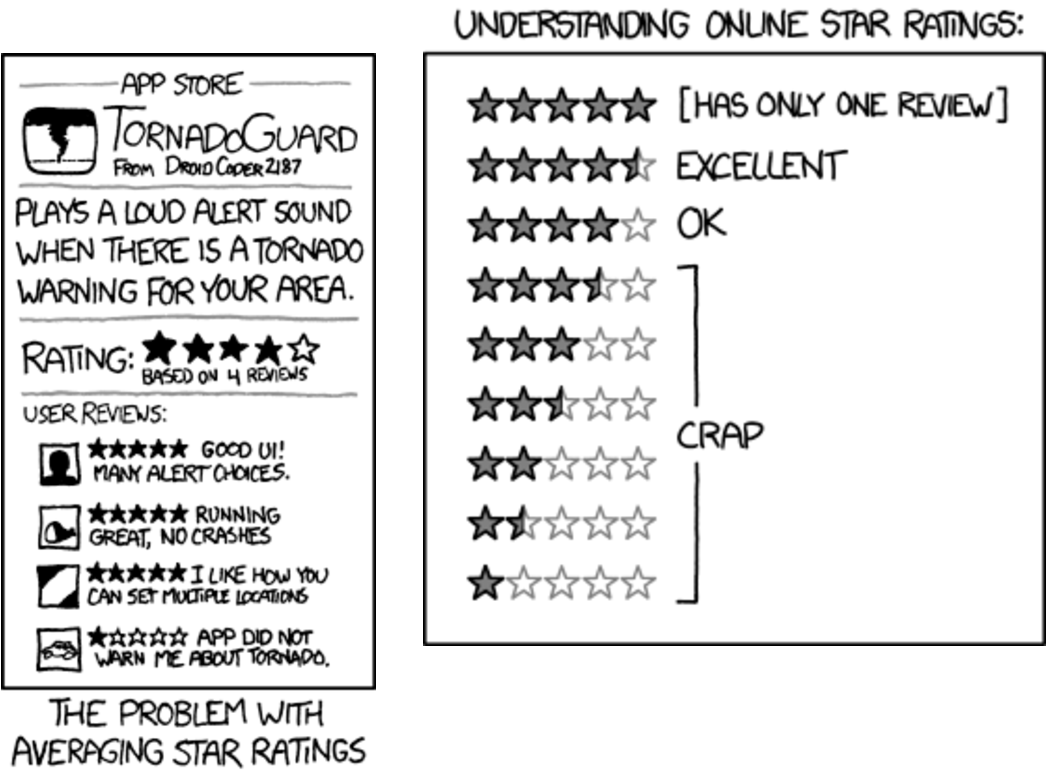
\includegraphics[width=\linewidth]{images/xkcd/xkcd-combined.pdf}
    \caption{XKCD's views on App Store Ratings and Reviews \\{\footnotesize Image sources: TornadoGuard \href{https://xkcd.com/937}{xkcd.com/937}, Understanding online star ratings \href{https://xkcd.com/1098}{xkcd.com/1098} \\ \href{https://creativecommons.org/licenses/by-nc/2.5/}{creativecommons.org/licenses/by-nc/2.5/}}}
    \label{fig:xkcd-app-store-ratings}
\end{figure}


Gaming ratings includes activities such as an app first asking if a user is happy with the app, and if they say yes then providing a link to encourage the user to rate the app positively in the app store.  An illustrative industry case study explained how Novoda improved the rating of a major newspaper's app using similar techniques~\sidecite{novoda_akan2016_asking_for_app_feedback_the_effective_way}. And in terms of the \Glspl{sdk} developers can use for in-app feedback, \myindex{Apptentive} is one of several companies that provides SDKs to help developers optimise their ratings and reviews and guides on how to do so within a mobile app~\sidecite{walz2015_apptentive_the_mobile_marketers_guide_to_app_store_ratings_and_reviews}. Unsurprisingly, ratings are also a subject of research interest.\sidenote{I,R,123456,C,G}

Here are several representative papers that focus on engineering aspects of ratings and reviews.  \citeauthor{alsubaihin2019app_store_effects_on_software_engineering} discusses the symbiotic relationship between releases and the ratings and reviews that app received~\sidecite[][p. 14]{alsubaihin2019app_store_effects_on_software_engineering}. Some developers time their releases based on the feedback they've received and monitor ratings and reviews for their latest release to influence the rollout of the new release. There have been innovative ideas on using ratings to prioritise software engineering activities including software testing of Android games apps~\sidecite{khalid2014_prioritizing_the_devices_to_test_your_app_on_casestudy_android_games}. And in \citeauthor{greenheld2018_automating_developers_responses_to_app_reviews} the value of developers responding to reviews was highlighted~\sidecite{greenheld2018_automating_developers_responses_to_app_reviews}.\sidenote{I,R,123456,C,G} 

In a population of 10,000 Android apps extracted from Google Play, correlations was identified between the density of warnings reported by \myindex{FindBugs}, a static analysis tool, and app store reviews and ratings for these apps~\sidecite{khalid2016_examining_the_relationship_between_findbugs_warnings_and_app_ratings}. They considered three warning categories: bad practices (which include reports of crashes in the reviews), internationalisation, and performance (which might relate to \Glspl{anr}, however they didn't investigate this aspect). They did not investigate whether addressing warnings from FindBugs improved the ratings or reviews for those apps, and mobile analytics was not mentioned in their work - unsurprising as they took a black box approach using decompiled Android app binaries.\sidenote{I,R,123456,C,G}

Via Figure \ref{fig:xkcd-app-store-ratings} XKCD aptly sums up two facets of flaws in app store ratings and reviews, averaging reviews may not be a good measure~\sidecite{explainxkcd_937_tornadoguard}, and the star ratings are not treated as a linear scale in practice~\sidecite{explainxkcd_1098_star_ratings}. In summary, app Store ratings therefore may not be an ideal measure of the quality of an app from a software engineering perspective!\sidenote{I,R,123456,C,G}
% See also stanik2020_requirements_intelligence_on_the_analysis_of_user_feedback
% shen2017_towards_release_strategy_optimization_for_apps_in_google_play 

\FloatBarrier

\subsection{Reviews in app stores}~\label{rw-reviews-in-app-stores}
Similarly reviews in app stores have been analysed for various purposes including for complaints and bug reports. Of the many and various research on reviews of mobile apps in app stores. 
Two early papers, the first focusing on Android apps in Google Play~\textcite{fu2013_why_people_hate_your_app_making_sense_of_user_feedback_in_a_mobile_app_store} and the second for iOS apps in Apple's App Store~\textcite{khalid2015_what_do_mobile_app_users_complain_about}.\sidenote{I,R,123456,C,G}

In \textcite[p. 5][]{fu2013_why_people_hate_your_app_making_sense_of_user_feedback_in_a_mobile_app_store} the top three most common indicators of problems in the apps were: slow 9,939, crashes 9,081, and freezes 3,960. Stability was a common theme of complaints about both free and paid apps [pp. 7-9].\sidenote{I,R,123456,C,G}

In \sidecite{khalid2015_what_do_mobile_app_users_complain_about} clearly establishes connections between what users of \myindex{iOS} apps complain about and the effects of these complaints on ratings of those apps; and \sidecite{panichella2015_how_can_i_improve_my_app_classifying_user_reviews_for_sw_maintenance_and_evolution} extends that work to consider the relevance of various review-topics to developers. Panichella \emph{et al} also extend the work to include Android apps in the Google Play Store. \sidecite{mcilroy2016_analyzing_and_automatically_labelling_the_types_of_user_issues_raised_in_mobile_app_reviews} - labels the content of reviews extracted from Google Play and found crashes and crashing were one of the topics that was a) relatively easy to categorise, and b) occurred frequently. This paper seemed to conflate in-app analytics tools (Flurry)\index{Flurry Analytics} with analytics of reviews (\emph{e.g.} \myindex{AppAnnie}). As an observation, since this paper was published Google Play now provides automated labeling and analysis of reviews.\sidenote{I,R,123456,C,G}

One of the curiosities reported in~\sidecite[][p. 13]{alsubaihin2019app_store_effects_on_software_engineering} is: \emph{``while automatic in-app crash reporting is the most prolific channel of reporting bugs, the one mostly prioritised by our respondents is user reviews in app stores.''} What are the effects of the crashes being a lower priority than user reviews? Also, they don't discuss other sources of crash reports (\emph{e.g.} platform crash reporting) even though these existed at the time of their research.\sidenote{I,R,123456,C,G}

Similarly, in terms of managing releases in app stores, the platform provided release management tools and reports were not mentioned in research, perhaps as few researchers even know of their existence? and they are not well-publicised or described, for example they are alluded to in a Play Console help article, \emph{``In Play Console, you can see an overview of your app's ratings, individual user reviews and clustered data about your app's reviews.''}~\sidecite{google_play_view_and_analyze_your_ratings_and_reviews} without further detail.\sidenote{I,R,123456,C,G}

Feedback comes in various forms, ratings and reviews are only two of them.  One that's seldom used in industry and seldom researched is implicit feedback recorded through user-interactions with the GUI of the mobile app. Common terms for this mechanism include `\glspl{glossary-heatmap}' and `heatmapping'\index{Heatmaps} and there are commercial \Glspl{sdk} and opensource projects available that perform the recording within an app at runtime. The elixir of automating `record and playback' test automation sometimes uses similar methods to record the interactions with a mobile app.\sidenote{I,R,123456,C,G} 

\subsection{In-app feedback}~\label{rw-in-app-feedback-topic}
Several papers discuss in-app feedback with the aim of helping developers. 

The first is a mapping study that aimed to identify the requirements for in-app feedback tools to support in-app feedback to improve the quality of apps. After various filtering they selected 36 papers. They analysed and categorised the types/forms of feedback, \emph{e.g.} text, audio, video, [file] attachments, and even emotions and behaviour. They also determined whether feedback was initiated by the user or by the app~\sidecite{scherr2022_the_way_it_made_me_feel_creating_and_evaluating_in_app_feedback_etc}. 
They created and testing their implementation of in-app feedback using an app designed for Citizens to provide feedback to a smart city project. Their test was performed with friends and colleagues of the team so not likely to be representative in terms of the content or behaviours. Nonetheless their research and their prototype in-app feedback may be of interest to app developers in future, especially given their analysis of how to design the feedback.\sidenote{I,R,123456,C,G} 

The paper did not mention software analytics nonetheless their app might include in-app-software analytics.\sidenote{I,R,123456,C,G}

The final paper for this section I co-wrote~\sidecite{avellis_harty_yu_towards_mobile_twin_peaks} where we proposed in-app, bi-directional feedback to help developers and users communicate requirements. This short paper does introduce mobile analytics as a complementary source of information.\sidenote{I,R,123456,C,G} 


\subsection{Testing}~\label{rw-testing-topic}
Testing for mobile has already been covered in \secref{rw-testing-mobile-apps-topic}. Here the focus is on feedback aspects of the testing.\sidenote{I,R,123456,C,G}

The absence of automated tests does not prove developers do not test their Android apps, rather it indicates their projects are unlikely to have any automated tests and similarly that the project is unlikely to run any automated scripted tests as part of a continuous build. (In honour of Dijkstra's observation that ``Testing shows the presence, not the absence of bugs'', Edsger W. Dijkstra in ~\sidecite[][p. 16]{randell1970_software_engineering_techniques_nato_dijkstra}.)\sidenote{I,R,123456,C,G} % Found via https://en.wikiquote.org/wiki/Edsger_W._Dijkstra
% See also: https://www.techwell.com/techwell-insights/2018/12/can-we-ever-find-all-bugs 
% https://wiki.c2.com/?TestsCantProveTheAbsenceOfBugs



\emph{``Thus even if the app is tested on one device, there is no guarantee that it may work on another device."}~\sidecite[][p. 27]{nagappan2016_future_trends_in_sw_eng_for_mobile_apps} - I agree. Sadly, they did not provide any evidence for this statement.\sidenote{I,R,123456,C,G}

And yet, researchers also continue to complain app developers don't test their apps sufficiently. They sometimes berate the app developers to `test their apps' ,\emph{e.g.}~\sidecite{cruz2019_guess_what_test_your_app}.
Similarly the voices of the researchers seem to go unacknowledged and unapplied.\sidenote{I,R,123456,C,G}

Another strand is where researchers collate examples of apps together with faults they have identified and analysed in order to help, primarily, other researchers.\sidenote{I,R,123456,C,G} 

Why are all these efforts to improve software testing for mobile apps generating seemingly minimal effects in practice? Perhaps researchers interested in improving mobile apps would find an approach similar to the research of~\sidecite{winter2022_lets_talk_with_developers_etc_automatic_program_repair} more productive - by actually talking \emph{with} the app developers and then offering to research pain points identified by those app developers. Doing so might increase the external and ecological validity of the research and potentially also increase the adoption of the research. The adoption might be at an individual developer, team, or organisation level. In some instances the effects of the research may gain wider adoption and become a tool, technique, approach that many app developers adopt. In some cases the app store and/or platform provider might also adopt the work, for instance to replace their current `Monkey'\index{Android Test Automation!Monkey} test tool. As an aside Google already has replaced their `Monkey' utility with `robo'\index{Android Test Automation!Robo}.\sidenote{I,R,123456,C,G}

The is evidence that developers do want automated tests and tools to provide them with feedback~\sidecite[][p. 5]{greiler2022_an_actionable_framework_for_understanding_and_improving_developer_experience} even if relatively few projects have sufficient tests to provide the developers with a level of comfort and confidence. Again, much of the research has focused on where researchers can find tests rather than working with development teams to understand their desires and the barriers that mean the developers don't have (m)any tests.\sidenote{I,R,123456,C,G}

For project teams with large volumes of automated tests, what value do those tests provide in terms of feedback about the quality of the app they are intended to test? Fortuitously one of the app-centric case studies explored in this research, Catrobat, has an opensource codebase and their uses of automated tests are well researched. The \myindex{Catrobat} project makes extensive use of various forms of automated tests including using \Gls{bdd} practices~\sidecite{ali2019using_catrobat}, testing under adverse conditions~\sidecite{adamsen2015systematic_catrobat}, the use of sizing for automated tests~\sidecite{hirsch2019approach_catrobat}, \emph{etc}.\sidenote{I,R,123456,C,G} % TODO add additional references for Catrobat. See the findings-results chapter.

Despite this investigation of testing in the literature, there is limited evidence that provides an understanding of the mobile app developers' perspective of testing practices, how tests interact with other information available to developers and the overall impact on mobile app quality.\sidenote{I,R,123456,C,G}

\subsection{Mobile Analytics}~\label{rw-mobile-analytics-topic}
In-app analytics have been used to help developers understand ways their mobile app is used by large populations of end-users and the effects of various conditions on the behaviours of the end users. There has been some research into using mobile analytics to understand usage patterns of specific apps.\sidenote{I,R,123456,C,G}

The first two of these papers focused on aspects of usability and on helping developers understand the users  of their app.

\newthought{Using Google Analytics to improve usability testing: }
\myindex{Google Analytics} for Mobile Applications was used to provide continuous usability logging to address challenges and severe limitations with usability testing in the lab. They prescribed a three-stage approach for logging. In the third stage they have two alternatives, one for lab usability testing, the other for continuous usability logging using Google Analytics.~\sidecite{ferre2017_extending_mobile_app_analytics_for_usability_test_logging}.\sidenote{I,R,123456,C,G}

\newthought{Helping devs understand the users of their app: }
Automatic instrumentation of mobile apps using mobile analytics tools including HP's \myindex{App Pulse Mobile} was able to help developers better understand their users~\sidecite{parate2016_RECKON_an_analytics_framework_for_app_developers_HP_AppPulseMobile}.\sidenote{I,R,123456,C,G}

Neither of these publications considered using mobile analytics for other purposes.

\newthought{Using mobile analytics to improve mobile apps: }
Two mobile apps incorporated a toolkit library called Insight\index{Insight (Analytics)} that combined passive analytics, such as session length, with factors, such as network condition and client device, with the aim of helping the developers recognise correlations between these factors and application use and revenues~\sidecite[][p. 82]{patro2015_building_blocks_to_understand_wireless_experience}. (Interim aspects of this research was also published by~\sidecite{patro2013_capturing_mobile_experience_in_the_wild} in 2013.)\sidenote{I,R,123456,C,G}

The research describes generic data, collected by Insight\index{Insight (Analytics)} for any app, and app-specific data, which is defined and implemented by the developers of that app~\sidecite[][pp. 87-88]{patro2015_building_blocks_to_understand_wireless_experience}. They identified a correlation between battery drain and session lengths; As battery drain increased the session lengths decreased. They also identified a correlation between screen brightness and battery drain. The device model was a material factor in the rate the battery drained, and in particular on Kindle Fire devices the drain was far higher when the screen was bright. ``\emph{controlling the screen brightness on a Kindle Fire device reduced the average battery drain by 40\% while using SB}''~\sidecite[][p. 13]{patro2015_building_blocks_to_understand_wireless_experience} Note: SB is short for StudyBlue, one of the two apps in their study.\sidenote{I,R,123456,C,G}

The research using Insight\index{Insight (Analytics)} was one of the catalytic agents for this research as it was able to publish data obtained using mobile analytics for two popular real-world apps. 
They also made both their client~\sidenote{\href{https://github.com/patroashish/InsightClient}{github.com/patroashish/InsightClient}} and server~\sidenote{\href{https://github.com/patroashish/InsightServers}{github.com/patroashish/InsightServers}} code freely available online as opensource projects. 
Although they mention they developed an iOS SDK it does not appear to have been made available online~\sidecite[][p. 85]{patro2015_building_blocks_to_understand_wireless_experience}.\sidenote{I,R,123456,C,G}

Perhaps paradoxically the Insight\index{Insight (Analytics)} client \Gls{sdk} does not record or report any failures of the SDK or of the associated app it has been integrated with. Assuming crashes, freezes, and other similar issues might affect the end-user experience it seems odd the SDK doesn't track these aspects. Furthermore the SDK only sends the analytics data when there is a working mobile network immediately available, it does not appear to queue events, incorporate any robustness mechanisms, or include any re-transmission capabilities.\sidenote{I,R,123456,C,G}

In their research they provided only a brief comparison between Insight\index{Insight (Analytics)} and three then popular mobile analytics services. Their brief comparison did not go into any detail about the characteristics or use of those three services.\sidenote{I,R,123456,C,G}

There has been research into various risks and concerns when using mobile analytics. Here is research that provides pertinent advice for app developers, and other stakeholders on how to improve end-users' privacy when incorporating in-app mobile analytics.\sidenote{I,R,123456,C,G}

5.2\% of app developers of top Android apps in Google Play have violated either their own privacy policy or the terms of service of the mobile analytics service they use in their app~\sidecite{zhang2020_how_does_misconfiguration_of_mobile_analytics_services_compromise_mobile_privacy}. This number may be an underestimate as method the researchers used (decompilation of the application's binary file) did not work on obfuscated binary files as top (\emph{i.e.} popular?) apps~\sidenote{The authors did not define what a top app is.} are like to be protected through obfuscation. The advice to app developers in this research is pertinent - they should abide by both their own privacy policy and by the terms of service of the analytics services they use.\sidenote{I,R,123456,C,G}

%This has similarities to earlier research \emph{``Alde: privacy risk analysis of analytics libraries in the android ecosystem."} published in 2016. In that paper they include apps available in China, a smaller data set of apps 100 from China, 200 from Google Play, and they use both static and dynamic analysis. They also created two phishing apps to demonstrate how PII data could be captured and recorded using mobile analytics. 10.1109/TMC.2019.2903186 seems to be a revised version of the 2016 paper with some additional code analysis techniques and an app to manage things. The following paper also discusses PII leaks in Android apps; it doesn't add much in terms of applicability to my research so I'm excluding it: \emph{``Bug Fixes, Improvements, ... and Privacy Leaks - A Longitudinal Study of PII Leaks Across Android App Versions."} 2018.

Note: there has also been research into similar sounding work on software analytics for mobile apps: an opensource project called \Gls{samoa}. However, their research investigated characteristics of the source code, rather than in the use of mobile analytics by app developers~\sidecite{minelli2013_software_analytics_samoa}.\sidenote{I,R,123456,C,G}

Chapter 33 in \sidecite[][pp. 177-187]{orosz2021_building_mobile_apps_at_scale} provides an industry perspective of the importance of [mobile] analytics, monitoring, and alerting. This book draws sources from experienced industry practitioners who have worked extensively with mobile apps from an engineering perspective~\sidenote{I was one of the people who contributed.}. The chapter explains how metrics are often wrong yet teams do not notice for years. It then presents the metrics certification process used at Pinterest which helped that company detect flaws with their mobile analytics, often before the analytics went live. Unmentioned, yet probably, Pinterest has developed in-house mobile analytics in order to apply their certification process.\sidenote{I,R,123456,C,G}

Research into mobile analytics is surprisingly rare, especially given the prevalence of apps that include mobile analytics SDKs and their use by mobile app developers. A possible reason for the rarity is the challenges in researchers obtaining access to the outputs of the mobile analytics. For the research into Insight analytics the researchers developed their own client SDK and server code and they negotiated special non-disclosure agreements (NDAs) and the data was pre-filtered to increase the privacy of the end users~\sidecite[][p. 91]{patro2015_building_blocks_to_understand_wireless_experience}. This provided them with access to the analytics outputs. Their research did not investigate third-party mobile analytics services or go into details of how developers applied the mobile analytics to effect improvements to the apps or related artefacts.\sidenote{I,R,1234,C,G}

Before we leave the topic of mobile analytics, research into the privacy aspects of the mobile analytics \Glspl{sdk} is pertinent as the choices developers make in terms of selecting in-app mobile analytics has various consequences. These consequences include the privacy for the end users who indirectly provide the underlying data. Two illustrative areas of research into the privacy and data leakage aspects are:\sidenote{I,56,C}

\begin{itemize}
        \item A privacy-focused app is used to obtain the network traffic sent to ad and analytics end points from end-user devices. That traffic is analysed to understand where it goes, who has access to the underlying data, and what of the content is most likely to contravene ePrivacy and GDPR directives\cite{razaghpanah2018_apps_trackers_privacy_and_regulators_a_global_study_of_the_mobile_tracking_ecosystem}.
        \item In contrast, the binary files of various apps were modified in order to intercept the calls to the respective in-app \Glspl{sdk} of various mobile analytics libraries. They developed a proof-of-concept Android app AlManager that a) allowed the user to see the contents of the calls made to the in-app SDKs, and b) blocked or replaced the contents with blank data. They also studied characteristics of the calls the apps made in terms of the App, Activity, and User level in terms of the data being sent to the mobile analytics SDK(s)\cite{liu2020_privacy_risk_analysis_and_mitigation_of_analytics_libraries_in_the_android_ecosystem}.
\end{itemize}

The first of these papers focused on the data that is sent, the contents, and where that data goes. The second concentrated on analysing app binaries to find all the calls to the mobile analytics SDKs. It then intercepted these and enabled users to see, block, or blank out data that would then be sent by the respective mobile analytics \Gls{sdk}.\sidenote{I,35,C}

Finally in terms of research into mobile analytics there is a paper that initially appeared relevant as their research was on software analytics for mobile apps. They describe a web-based software analytics platform named \Gls{samoa}\index{SAMOA}\sidecite{minelli2013_software_analytics_samoa} that was developed to provide insights into the source code of various Android apps. They analysed opensource codebases for apps on \myindex{F-Droid}~\sidenote{\href{https://f-droid.org/}{f-droid.org/}}. While their analysis is of interest~\sidenote{And one of the authors kindly provided their source code.}, they did not investigate mobile analytics. (Also they researched apps on \Gls{glossary-f-droid}, however apps on F-Droid are not permitted to include mobile analytics unless all the SDK and libraries are also opensourced).\sidenote{I,R,3,C,G}
%%%% There's no succinct reference I can find, here are various bits and pieces on this topic:
% https://forum.f-droid.org/t/inclusion-and-foss-status-of-firebase-android-sdk/19172
% https://forum.f-droid.org/t/shouldnt-google-analytics-and-google-services-be-antifeatures/4991
% https://forum.f-droid.org/t/sky-map-integrating-google-firebase-analytics/19259

\subsection{Summary} % sources of information
Developers are faced with a plethora of sources of information. Some they choose, such as providing in-app feedback mechanisms and in-app mobile analytics. Others may be forced on them (and testing might be a mix of the two). There is some research into uses of mobile analytics, but little of substance on how it can be effectively used by developers to improve their practices and their apps. Also there is scant research into the mobile analytics tools and services in terms of the information they provide developers.\sidenote{I,R,134,C,G}

\section{Chapter summary}~\label{rw-summary-section}
App stores, their ecosystems, and their effects on developers have been covered from various angles. Some of the research describes snapshots of one or more app stores. And some of the research involves developers of live apps in a mainstream app store. Ratings and reviews are covered from many angles including fraud~\sidecite{xie2015_appwatcher_unveiling_the_underground_market_of_trading_mobile_app_reviews}. Yet few have investigated the use of mobile analytics.\sidenote{I,r,34,C,G}

Following on from a point raised earlier in this chapter: emph{``between detecting failures and achieving reliability.''}~\sidecite[][p. 77]{frankl1997choosing_testing_for_reliability}. Mobile Analytics might be able to provide a real-world measure in terms of achieving reliability. Furthermore, much of the research into mobile app crashes seems to end prematurely - before considering whether reliability of the app has been improved by whatever method and approach they have researched.\sidenote{I,R,1234,C,G}

\begin{quote}
    \emph{``...with explicit and implicit feedback now available (almost) continuously, questions arise. How can practitioners use this information and integrate it into their development processes to decide when to release updates?''}\sidecite[][pp. 48-49]{maalej2016_towards_data_driven_requirements_engineering}    
\end{quote}

Building on a point made in that paper: \emph{``the future of app quality engineering is data driven."}~\sidecite[][p. 24]{nagappan2016_future_trends_in_sw_eng_for_mobile_apps}. Mobile Analytics incorporates rich seams of data that may help developers perform app quality engineering. However, in order to help developers mine this data more effectively and process it into actionable information, we need a better understanding of current practices associated with using mobile analytics. This includes investigating how mobile analytics use is integrated into mobile development practices and the effects it has on the quality of the software artefacts associated with mobile apps. Further, we also need to understand the capabilities and limitations of existing mobile analytics tools. These gaps in our understanding lead to the six perspectives introduced in Chapter \secref{chapter-introduction} and the overarching research question for this thesis: \emph{How can applying analytics improve software development and software testing for mobile apps in practice?}\sidenote{I,123456,G}

The next chapter explains the methodology used in this research to identify and record ways developers use mobile analytics currently, the sources of pertinent data, and the approach this research took to answer the research questions.


%\julian{TODO complete this thought: However none of these (these researches) provide X which is my need...}